\documentclass{article}

% Language setting
% Replace `english' with e.g. `spanish' to change the document language
\usepackage[english]{babel}

% Set page size and margins
% Replace `letterpaper' with `a4paper' for UK/EU standard size
\usepackage[letterpaper,top=2cm,bottom=2cm,left=3cm,right=3cm,marginparwidth=1.75cm]{geometry}

% Useful packages
\usepackage{amsmath}
\usepackage{amsfonts}
\usepackage{bm}
\usepackage{graphicx}
\usepackage[colorlinks=true, allcolors=blue]{hyperref}
% \usepackage[numbers]{natbib}
\usepackage[natbib=true, style=ieee, doi=false,isbn=false,url=false,eprint=false]{biblatex}
\usepackage{csquotes}
\usepackage{multirow}
\usepackage[normalem]{ulem}
\usepackage{caption}
\usepackage{subcaption}
\usepackage{authblk}
\usepackage{gensymb}

\addbibresource{sample.bib}
\defbibfilter{appendixOnlyFilter}{
  segment=1 % Segment 1 will be chosen to be the one in appendix
  and not segment=0 % Default segment is 0
}

\title{China Outbound Tourism Forecasting amid COVID-19}
\author[1]{Zhi Qin Tan, Jiaxi Li, Yunpeng Li \\
Department of Computer Science, University of Surrey}
\date{}
\begin{document}
\maketitle

\begin{abstract}
Tourism forecasting plays a critical role in the tourism industry and enables strategic planning for diverse stakeholders. However, this is a difficult task as it is influenced by multiple factors such as economic trends, political stability and global crises. 
This work studies the effectiveness of traditional approaches such as Seasonal Autoregressive Integrated Moving Average (SARIMA) and modern machine learning models (e.g. decision tree and recurrent neural network (RNN)) in forecasting China's outbound tourism visitors to different destinations for the upcoming year given the historical tourism arrival data. Empirical results show that ensembling RNN models achieve the best performance in forecasting tourism arrivals amid COVID-19 compared to other methods.
% Traditional forecasting approaches such as Seasonal Auto Regressive Integrated Moving Average (SARIMA) models have considered the effect of seasonal change, but the escalating unpredictability and the rise of irregular events necessitate more flexible and adaptive models. This paper focuses on using two modern machine learning models, Decision Tree and Recurrent Neural Networks (RNN), to predict China's outbound tourism visitors for the upcoming year given the past several year’s tourism data from different countries, and comparing their performance with the classic SARIMA, for their potential to effectively capture and interpret these intricate data patterns. The experiment result indicates that the RNN could give the best performance and we use it as the target algorithm to do the final point forecast and the interval forecast.
\end{abstract}

\section{Introduction}
Tourism forecasting is an essential process due to the inherent dynamism and potential uncertainties within the global tourism industry \cite{hassani2017forecasting}. 
% As one of the most rapidly expanding sectors globally, it is influential in determining a country's gross domestic product (GDP). 
Accurate forecasting can guide various stakeholders including government bodies, private firms and tourists themselves to adjust and plan strategically for the future \cite{peng2014meta, chatziantoniou2016forecasting, shahrabi2013developing}. 

As tourism is influenced by multiple factors such as economic trends, political stability and most recently, global health crises, robust models are essential for tourism forecasting \cite{song2019review}. Significant events such as the COVID-19 pandemic, the 2003 SARS outbreak, and the 2008 global financial crisis have notably caused abrupt disruption or ``structural breaks'' in tourist arrival patterns across many destinations \cite{fotiadis2021good, dombey2004effects, sheldon2010global}. As a result, the time series data for tourist arrivals display patterns that are non-stationary, non-linear and complex. The additional layer of complexity added by the seasonality in tourism \cite{hyndman2018forecasting}, coupled with the perishability of many tourism services has made the task of forecasting tourism demand increasingly challenging. 

Over the years, researchers have developed various methodologies to address the unique challenges of tourism forecasting. Traditional approaches including Seasonal Autoregressive Integrated Moving Average (SARIMA) and exponential smoothing state space models, are known for their merit in dealing with seasonal data with regular patterns. Nonetheless, the frequency and significance of irregular events have increased the need for more flexible and responsive forecasting models where algorithms based on machine learning provide an avenue for capturing the complexity and interdependence of influencing factors within the tourism industry. 
% Whereas, the raised number of irregular events has underscored the need for more flexible and responsive forecasting models where the algorithm based on machine learning provides an avenue for capturing the complexity and interdependence of influencing factors within the tourism industry. 

% X proposes AGA-SSVR that hybridises the support vector regression (SVR) model with the adaptive genetic algorithm (AGA) and the seasonal index adjustment to forecast holiday daily tourist flow. The result shows that it outperforms the AGA-SVR and back-propagation neural network. Furthermore, X proposes to combine SSVR model with fruit fly optimization algorithm (FOA) while use single-step-ahead and multi-step-ahead which are two kinds of forecasting horizons to verify the forecasting it's performance. X develop a decomposition-ensemble approach based on the complete ensemble empirical mode decomposition with adaptive noise, data characteristic analysis, and the Elman's neural network model. The experiment result indicate it outperforms other models in both point and interval forecasts for different prediction horizons. 

In this work, we focus on the task of China's outbound tourism forecasting to multiple destinations around the globe amid the COVID-19 pandemic. We experimented with several models including SARIMA, decision tree and recurrent neural network (RNN) to compare their performance and suitability.
% This paper focuses on the recurrent neural networks RNN which are more suited for dealing with complex time series data, and we compare it with the baseline algorithm SARIMA and the decision tree. 
The rest of this study is organised as follows: The problem statement and the methodology used are introduced in the next section. The third section illustrates the experiment setup and the result. We discussed our findings and conclude them in the last two sections.

\section{Methodology}
% This section formally defines the problem and introduces the method in detail.
\subsection{Problem Statement}
Let $\mathbf{y} \in \mathbb{R}^{N \times 1}$ be a series of historical monthly Chinese outbound tourist arrivals for a destination, and $\mathbf{x} \in \mathbb{R}^{N \times d_x}$ be an associated set of explanatory variables where $y_i$ is the observed tourist arrivals from China at the $i$-th timestep, $N$ is the number of timesteps and $d_x$ is the dimension of the explanatory variables. The goal is to construct a model with the data $\mathbf{y}$, $\mathbf{x}$ to estimate $y_{N+1: N+H}$ where $H$ is the forecast horizon. The constructed model should predict both point forecasts and interval forecasts of 80\% confidence level. The dataset gives historical data for 20 destinations, each with varying $N$ and $H$ (e.g. Data for Australia are available from 01/1989 - 01/2023 and Czech from 01/2012 - 12/2022, while the forecast period is until 07/2024).
% Given a series of historical monthly Chinese outbound tourist arrivals to different destinations, $Y = \{y_i\}_{i=1}^T$ where $T$ is the number of months, the goal of this task is to forecast tourist arrivals, $F = \{y_i\}_{i=T+1}^{T+1+N}$ where $N$ is the forecast period. The dataset gives historical data for 20 destinations, each with varying $T$ and $N$ (e.g. Data for Australia are available from 01/1989 - 01/2023 and Czech from 01/2012 - 12/2022, while the forecast period is until 07/2024). In addition to point forecasts, interval forecasts of 80\% confidence level are also predicted. 

\subsection{Model and Algorithm}
Several models and algorithms have been considered for tourist arrival forecasting. This subsection provides a brief introduction to each method.
\subsubsection{Seasonal Autoregressive Integrated Moving Average}
SARIMA is an extension to the popular forecasting method Autoregressive Integrated Moving Average (ARIMA) for univariate time-series data by introducing a seasonal component for each element of ARIMA, namely seasonal autoregression (AR) order $P$, seasonal difference order $D$, seasonal moving average (MA) order $Q$ and the number of time steps for a seasonal period $m$. Briefly, in addition to learning the coefficients of ARIMA, SARIMA also learns the coefficients of the added seasonal components:
\[
y_t = \sum_{n=1}^p \alpha_n y_{t-n} + \sum_{n=1}^q \theta_n \epsilon_{t-n} + \sum_{n=1}^P \phi_n y_{t-nm} + \sum_{n=1}^Q \eta_n \epsilon_{t-nm} + \epsilon_t
\]
where $\boldsymbol{\alpha}$, $\boldsymbol{\theta}$, $\boldsymbol{\phi}$ and $\boldsymbol{\eta}$ are the coefficients of AR, MA, seasonal AR and seasonal MA. SARIMA is usually used for forecasting simple univariate problems and  serves as a baseline in our study.

\subsubsection{Decision Tree}
Decision tree (DT) \cite{decisiontree} is a supervised learning algorithm which can be used for regression or classification tasks. It has a flowchart style, hierarchical and tree structure consisting of root node, branches, internal nodes and leaf nodes. DT is constructed starting from the root node, optimally splitting into branches based on certain feature values iteratively until it reaches leaf nodes that output the final prediction. The strength of DT compared to classical machine learning approaches such as linear regression is its ability to learn non-linear relationships between the dependent and independent variables and hence is more flexible.

Random forest (RF) \cite{randomforest} is a variant of DT which employs both feature bagging and bootstrapping to create a ``forest" of decision trees. A subset of features and data is randomly sampled when creating each decision tree to minimize the risk of overfitting and reduce biases. The final prediction is ensembled by taking the average outputs of all the decision trees in RF.

Extreme Gradient Boosting (XGBoost) \cite{xgboost} is another variant of the decision tree ensemble learning algorithm. The idea of gradient boosting refers to the creation of a collectively strong model by combining multiple weak models. In particular, XGBoost trains an ensemble of shallow decision trees using the residual error of the previous model to fit the next model iteratively and the weighted sum of all the decision tree predictions is outputted as the final prediction.

\subsubsection{Recurrent Neural Network}
% Traditional feedforward deep neural networks usually do not work well in time series or sequential problem due to the fact that there is no mechanism in them that learn the temporal relationship between timesteps. 
Recurrent neural network (RNN) \cite{rnn} is a variant of deep neural networks that can retain information from the past for downstream tasks such as forecasting or classification. RNN incorporate the concept of ``memory" that stores hidden states of previous inputs and process them together with the current input to generate the next output of a sequence. However, vanilla RNN suffers from the vanishing gradient problem where during backpropagation, as the sequence length gets longer, the gradient becomes smaller towards earlier timesteps and results in a small contribution to parameter learning. To overcome this, two variants of RNN are created which introduces internal mechanism called gates to regulate the flow of information, namely long short-term memory (LSTM) \cite{lstm} and gated recurrent unit (GRU) \cite{gru}.

LSTM added a cell state that carries relevant information throughout the sequence and uses various gates to decide which information to store in it. The forget gate decides what to forget from the cell state while the input gate decides what values from the input to be remembered in the cell states. Lastly, the output gate decides what the next hidden state should be based on the current cell state. All gates output a vector with values between 0 and 1 which are then multiplied with other vectors (i.e. cell states, hidden states and input) to decide which information to forget or remember.

GRU is a newer RNN variant which simplifies the internal operation of LSTM by removing cell states. GRU only has two gates as opposed to three in LSTM, a reset gate and an update gate. The reset gate decides how much past information to keep in the hidden state while the update gate decides what information to forget and what new information to add to the hidden state. Figure \ref{fig:rnn} illustrates the architecture of LSTM and GRU.

In both variants, hidden states of RNN are initialised at the first timestep, usually by setting its value to zero. Even so, sometimes we may want to generate different forecast sequences by conditioning our predictions on certain conditions (i.e. generating different tourism forecast predictions given the destination). 
% This technique was introduced by \cite{conditionrnn} in an image caption generator to generate caption by conditioning on the input image. 
Based on the different conditions, the hidden states are initialised differently instead of always initialising them with zeros \cite{conditionrnn}. See \ref{appx:cond} for more details.

\begin{figure}[htbp]
     \centering
     \begin{subfigure}[b]{0.45\textwidth}
         \centering
         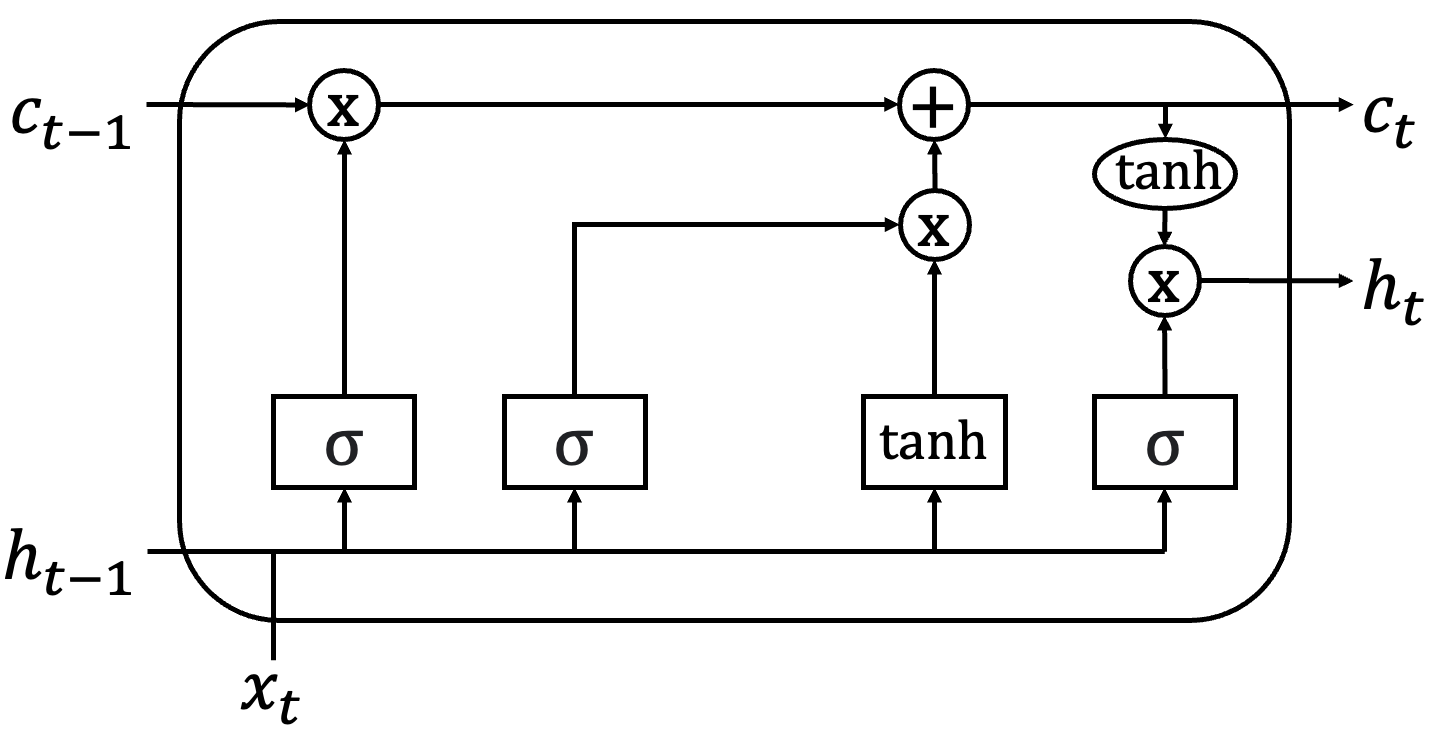
\includegraphics[width=.98\textwidth]{images/lstm.png}
         \caption{LSTM}
     \end{subfigure}
     \hfill
     \begin{subfigure}[b]{0.45\textwidth}
         \centering
         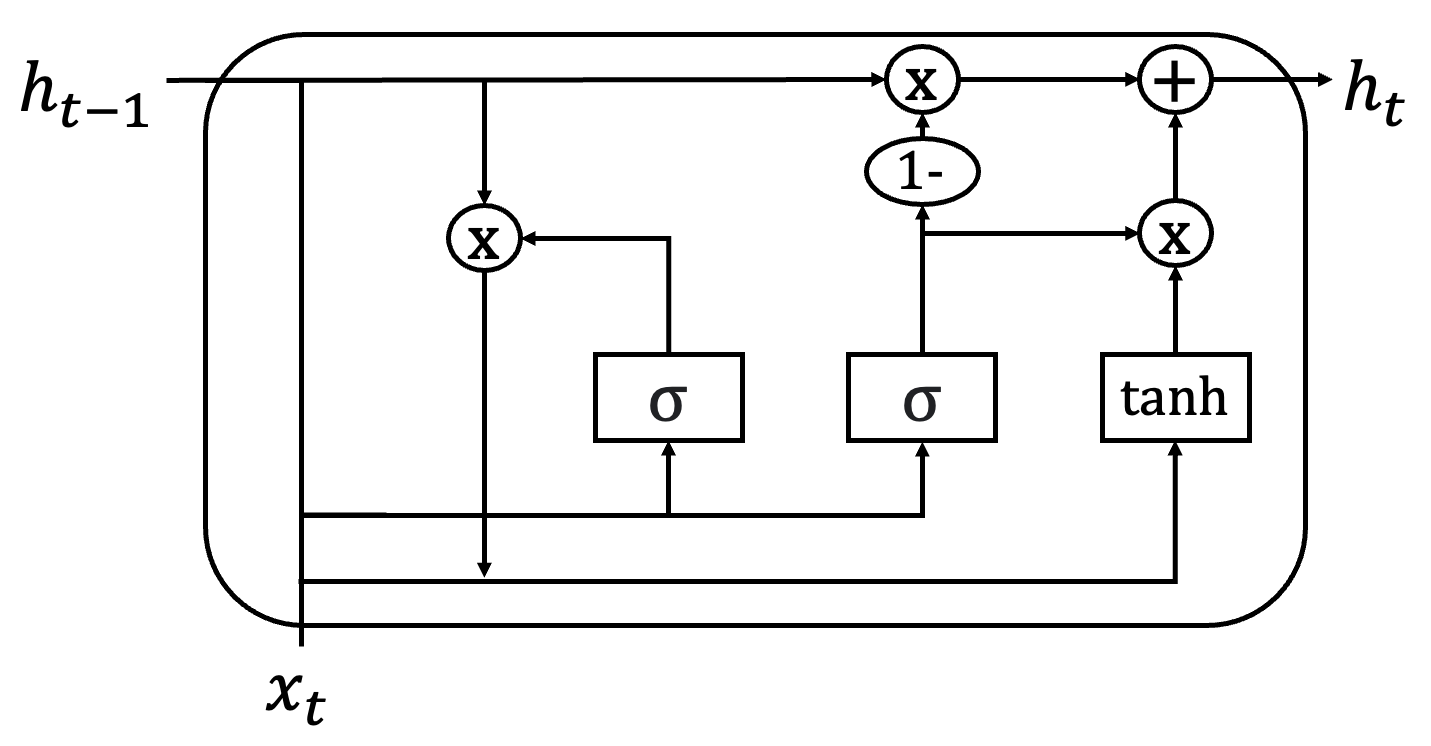
\includegraphics[width=\textwidth]{images/gru.png}
         \caption{GRU}
     \end{subfigure}
    \caption{Architecture of two RNN variants.}
    \label{fig:rnn}
\end{figure}

\subsection{Validation and Testing}
\label{sect:testing}
When building a model or selecting the best hyperparameters, we often need to evaluate its performance. Cross-validation \cite{cv1995} is the commonly used statistical method to achieve that. Traditionally, in K-Fold cross-validation, we split the training dataset into K folds, train the model on all folds except one and then evaluate the model on the excluded fold. We repeat this process for each fold and use the average performance across each repetition as our final metric. However, the K-Fold cross-validation technique is not suitable for time series forecasting as it makes no sense to use future values to forecast the past. In short, we must preserve the temporal relationship between the observations during cross-validation.

One way to perform cross-validation in time-series forecasting is to create training and validation splits on a rolling basis. For each cross-validation iteration, we slide the training and validation windows forward incrementally. This prevents the overlapping of validation data between each iteration while still preserving the temporal relationship of the observations. Figure \ref{fig:cvsplit} illustrates the rolling time series cross-validation method.

\begin{figure}[htbp]
     \centering
     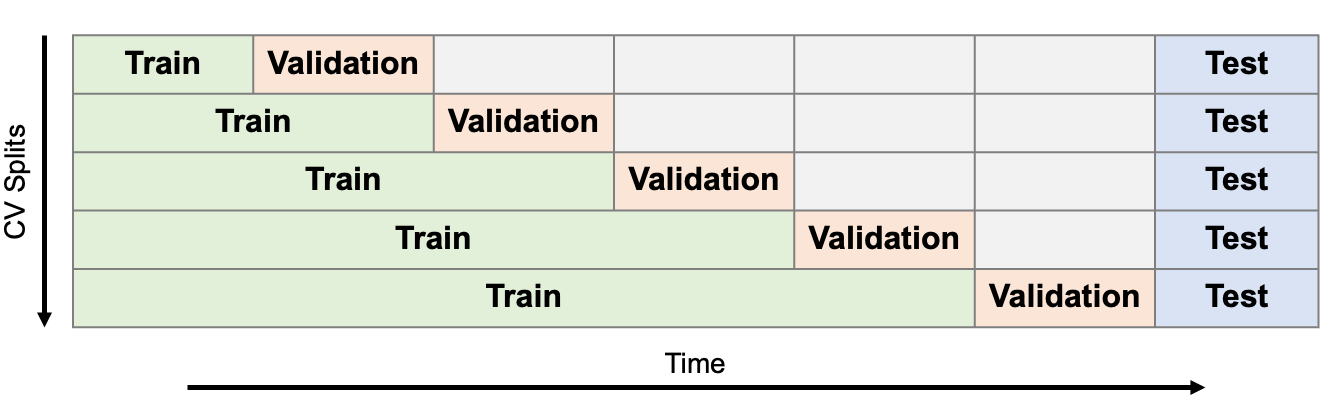
\includegraphics[width=.75\textwidth]{images/cv splits.png}
    \caption{Cross validation splits for time series problem.}
    \label{fig:cvsplit}
\end{figure}

\subsection{Feature Engineering}
% In the mathematical theory of deep neural network (DNN), the universal approximation theorem \cite{universalapp1989} says that given enough amount of data and parameters, a DNN can approximate any function as closely as we want. Loosely speaking, this means that DNN can figure out the composition of feature extraction and regression functions.
In general, given enough amount of data and parameters, a complex algorithm should be able to approximate any function as closely as we want. However, if we incorporate some feature engineering methods using domain knowledge, we can reduce the complexity of the model required for the problem and thus lower the risk of overfitting. 
Depending on the domain knowledge, we can create different features from explanatory variables (See \ref{appx:expvar}) that may be useful for tourism forecasting. This includes the percentage growth of GDP, the ratio and difference of GDP between each destination and the origin, the distance between each destination and the origin using geographic coordinates, etc.

In time series forecasting problems, temporal features such as month and year should also be fed into the prediction algorithm. We used cyclical features to encode periodical temporal features such as the month number as follows:
\[
M_{\sin} = \sin (2 \pi (n_m-1)/12)
\]
\[
M_{\cos} = \cos (2 \pi (n_m-1)/12)
\]
where $n_m \in \{1...12\}$ is the month number. Both $\cos$ and $\sin$ form unique pairs of values for each month number (See \ref{appx:ablation} for ablation studies). Figure \ref{fig:monthfeat} shows the periodicity of the encoded month number features.

\begin{figure}[htbp]
     \centering
     \begin{subfigure}[b]{0.4\textwidth}
         \centering
         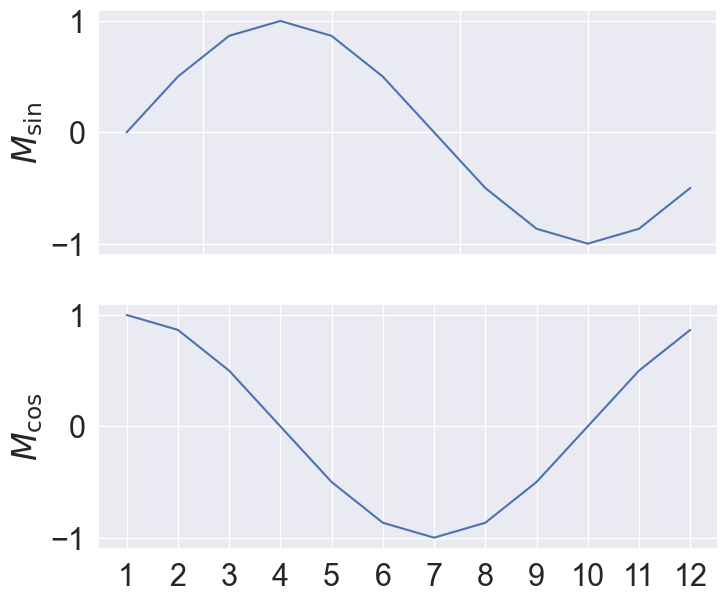
\includegraphics[width=\textwidth]{images/sine cosine.png}
         \caption{Encoded $M_{\sin}$ and $M_{\cos}$ feature.}
     \end{subfigure}
     \begin{subfigure}[b]{0.4\textwidth}
         \centering
         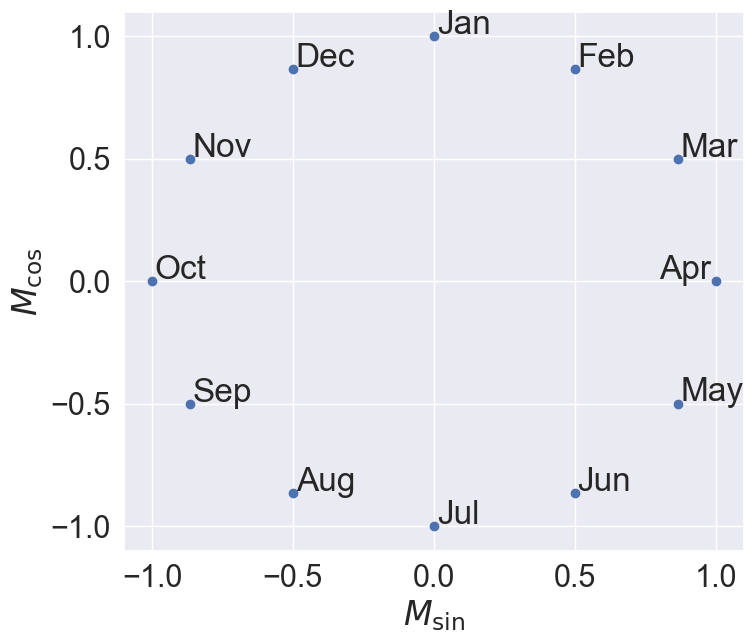
\includegraphics[width=\textwidth]{images/cyclic month.png}
         \caption{Unique feature pairs for each month.}
     \end{subfigure}
    \caption{Encoding periodic temporal features with $\sin$ and $\cos$.}
    \label{fig:monthfeat}
\end{figure}

% Additionally, the ``Popularity" feature is introduced by taking the median visitor arrivals of each destination as popular destinations may exhibit different trends compared to unpopular ones. A dummy feature ``Travel Restriction" is created by considering both the travel restriction of origin (China) and each destination. 

Lastly, certain assumptions have been made for the forecast period including: (1) all COVID-19 related variables will become exponentially less important towards the end of the forecast period; (2) Travel ban or border control is assumed to not happen again during the forecast period; (3) Static variables such as geographic coordinates or relative distance between origin and destination is constant throughout the whole time period. Missing or future values of explanatory variables (e.g. FSI and climate) and forecast variable (e.g. missing tourist arrival data from March to December 2013 in the Maldives) are imputed or projected using classical methods like exponential smoothing or SARIMA.

\subsection{Shocks and Unforeseen Events}
\label{sect:shocks}
Shocks in time series forecasting refer to the event where the time series data deviates quickly from a previous trend due to unexpected external events. These shocks exist in the historical data and must be accounted for before feeding into any model or algorithm. Though, we will assume that there will be no shocks when forecasting future visitor arrivals as these events are unpredictable. Figure \ref{fig:shocks} demonstrates a few examples of identified shocks. We used dummy variables ``Unrest" and ``Travel Restriction" to represent the shocks that were identified in the historical data.

\begin{figure}
     \centering
     \begin{subfigure}[b]{0.52\textwidth}
         \centering
         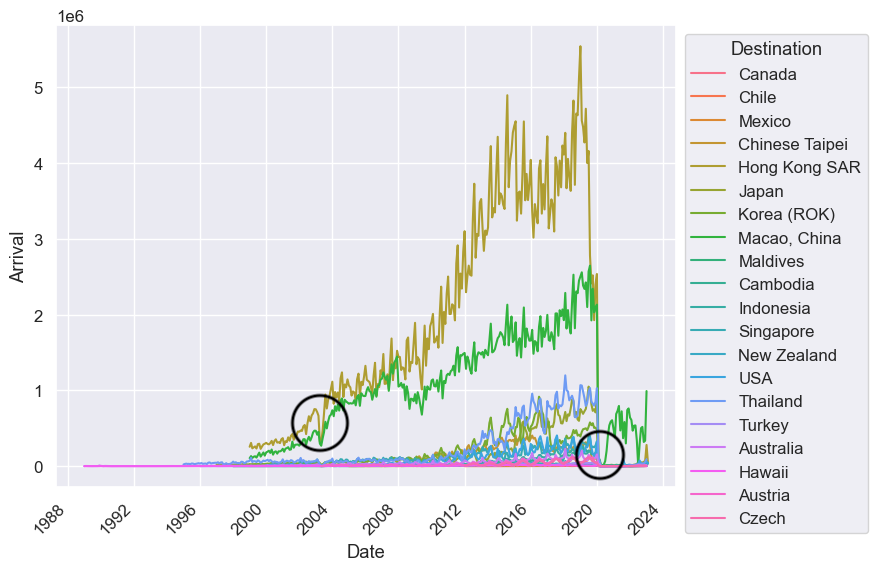
\includegraphics[width=\textwidth]{images/pandemic shock.png}
         \caption{Drop in visitor count globally due to SARS 2003 and COVID-19 pandemic.}
     \end{subfigure}
     \begin{subfigure}[b]{0.43\textwidth}
         \centering
         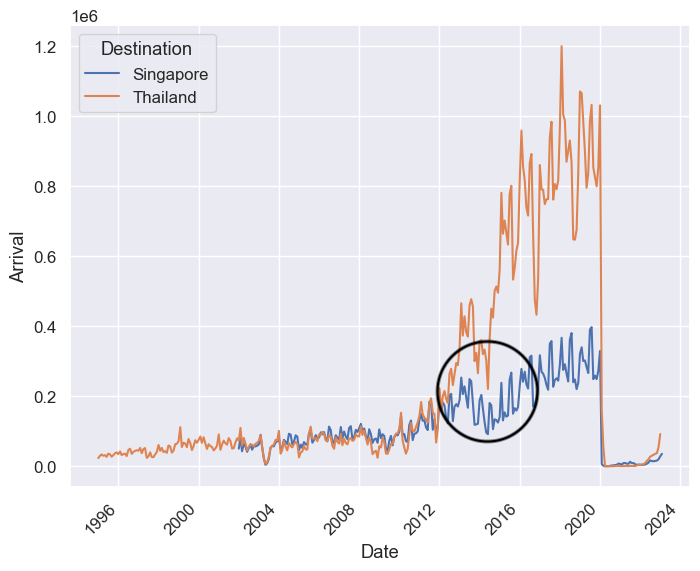
\includegraphics[width=\textwidth]{images/plane accident shock.png}
         \caption{Airplane crashes of Malaysia Airline affecting tourism in nearby destinations in 2014.}
     \end{subfigure}
    \caption{Examples of shocks and unforeseen events affecting tourism.}
    \label{fig:shocks}
\end{figure}

\subsection{Point Forecast}
Point forecast refers to the commonly known forecast problem where one exact value is predicted for each forecast timestep. For the baseline SARIMA, separate models are trained for each destination. For decision tree which is designed for regression problems, we can simply predict the dependent variable using the independent variables at each timestep and ignore the time dimension of the data. However, this will usually result in worse overall performance. A quick hack to introduce the time dimension is to create additional features by using the lagged value of the dependent variable (e.g. tourist arrivals at $t-1$). 

For RNN models, the typical way to generate point forecasts is to generate prediction one timestep at a time and then the current prediction is used as input to produce the next prediction. This process is repeated until a desired length of forecasts is acquired. The advantage of this method is that the model can utilize future explanatory variables (either made available with assumption or projection) for prediction. However, this method is numerically unstable as prediction is generated autoregressively and the prediction error is propagated through each subsequent timestep. Alternatively, if the forecast period, $H$ is known beforehand, we can design the RNN model to predict all $H$ predictions at once. This method is more stable but results in lesser training instances (i.e. only data up to $N-H$ timestep is usable). 
% To benefit from these two methods, we can ensemble them by taking the mean of their respective forecast predictions.

\subsection{Interval Forecast}
Interval forecast refers to the forecasting problem where a lower limit, $l_t$ and upper limit, $u_t$ with a confidence level $c$ are predicted. We used the idea of dropout as a Bayesian approximation \cite{bayesiandropout} since it is a quick and easy to implement technique. In neural networks, dropout is a well-established method to reduce overfitting and add regularization introduced by \cite{dropout}. Particularly, during the forward pass of a neural network, neurons in each layer are randomly dropped with a predefined probability. Usually, this is performed during the training stage only but \cite{bayesiandropout} has shown that with dropout enabled during inferencing, multiple passes of the neural networks are equivalent to Monte-Carlo sampling. With the sampled predictions, we can then approximate the prediction interval with
\[
l_t = \mu_t - z_{c}\sigma_t, \ \ u_t = \mu_t + z_{c}\sigma_t
\]
where $z_{c}$ is the critical z value for confidence level $c$, $\mu_t$ and $\sigma_t$ are the first and second moment of the samples at time $t$.

\section{Results}

\subsection{Experiment Settings}
We experimented with several models: (1) SARIMA as baseline; (2) DT model with lagged features; (3) RNN$_1$ model which generates forecasts autoregressively; (4) RNN$_{H}$ which predicts $H$ forecasts at once; and (5) RNN$_e$ which is an ensemble between RNN$_1$ and RNN$_{H}$. Two experiments setting were considered. Experiment 1 involves only tourism data from the pre-COVID period where we train models on data up to 2019 and use 2019 as testing data. This experiment is mainly used for model selection and hyperparameter tuning as it is unaffected by the volatility during the pandemic. Experiment 2 uses data up to 2022 and 2022 data as training and testing data respectively.

\subsection{Training Details}
For each experiment, the training data is further split into 5 folds to perform cross-validation and hyperparameter tuning using grid search (See \ref{appx:params}). Since machine learning algorithms usually converge faster when data is preprocessed to have similar scales, we performed log-transform on the dependent variable and standardised all variables so that they have 0 mean and standard deviation of 1. Standardisation is performed separately for each time series so that the variables are scaled relative to the destination. Next, although in theory, RNN is capable of learning seasonality, it is often better to remove periodical patterns from the time series data before feeding into the model using seasonal trend decomposition based on Loess (STL) \cite{stl} with seasonality during COVID-19 period (i.e. 2020-2023) set to 0. Finally, all preprocessing steps are inversely applied to the model output in reverse order to compute the final forecast. Figure \ref{fig:preprocess} demonstrates how log-transformation and standardisation unskew the data and Figure \ref{fig:stl} shows the effects of removing seasonality using STL. The models are trained by optimizing a MASE loss function (See \ref{appx:metric} for formula) while the weights of RNN are initialised using the Xavier initialisation method \cite{xavier}. Besides that, 100 trials of Monte-Carlo sampling with Bayesian dropout are drawn to approximate the prediction interval for RNN models.

\begin{figure}[htbp]
     \centering
     \begin{subfigure}[b]{0.45\textwidth}
         \centering
         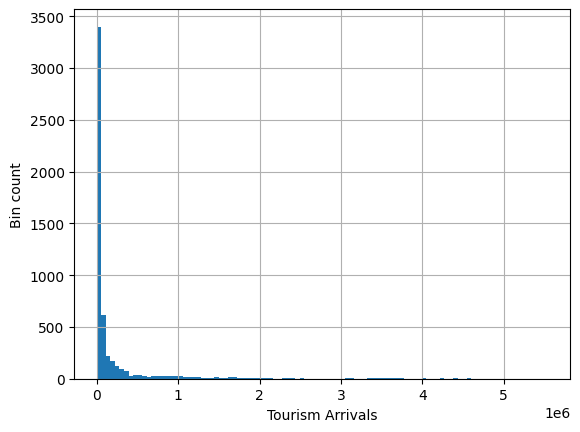
\includegraphics[width=\textwidth]{images/target before.png}
     \end{subfigure}
     \begin{subfigure}[b]{0.45\textwidth}
         \centering
         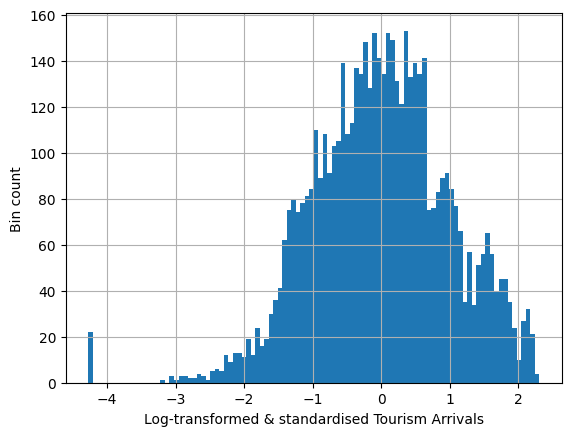
\includegraphics[width=\textwidth]{images/target after.png}
     \end{subfigure}
    \caption{Histogram of tourism arrivals for all destinations before and after the preprocessing steps.}
    \label{fig:preprocess}
\end{figure}

\begin{figure}[htbp]
     \centering
     \begin{subfigure}[b]{0.45\textwidth}
         \centering
         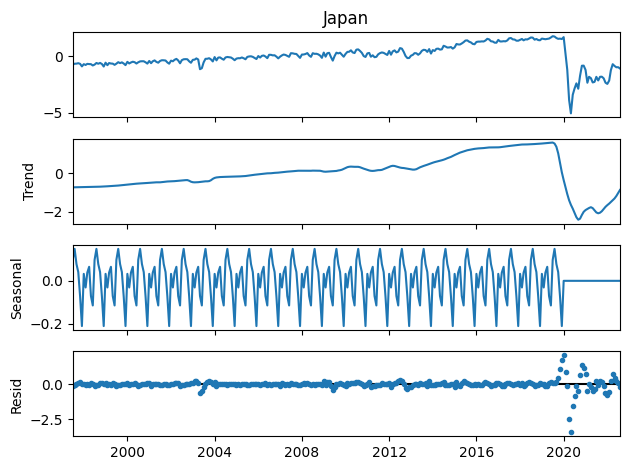
\includegraphics[width=\textwidth]{images/stl.png}
         \caption{STL decomposition of tourism arrivals with seasonality explicitly set to 0 between 2020-2023.}
     \end{subfigure}
     \begin{subfigure}[b]{0.45\textwidth}
         \centering
         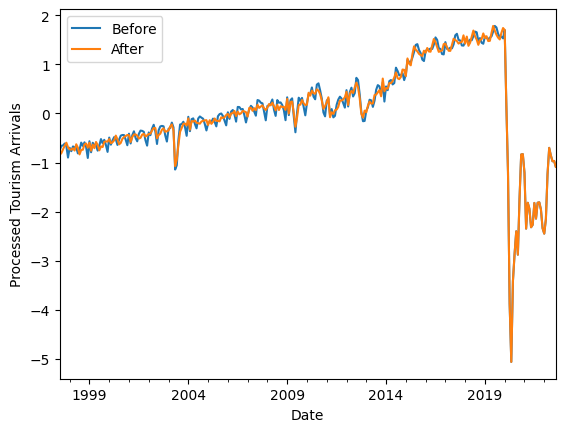
\includegraphics[width=\textwidth]{images/seasonality removal.png}
         \caption{Sesonality removal with STL.}
     \end{subfigure}
    \caption{Effects of removing seasonality with STL of tourism arrivals in Japan.}
    \label{fig:stl}
\end{figure}

\subsection{Experimental Results}
To evaluate the performance of our models, we used root mean squared error (RMSE), R2 score, mean absolute error (MAE), mean absolute percentage error (MAPE) and mean absolute scaled error (MASE) \cite{hyndman2006} as evaluation metrics for point forecast while mean Winkler score \cite{winkler} is used to evaluate interval forecast. See \ref{appx:metric} for more details. Table \ref{table:expres} shows the testing performance of each model in both experiments. Figure \ref{fig:expres} illustrates the forecast prediction and actual ground truth for both experiments.

\begin{table}[htbp]
\small
    \centering
        \begin{tabular}{l|l|cccccc}
            Experiment & Model & RMSE ($\downarrow$) & R2 ($\uparrow$) & MAE ($\downarrow$) & MAPE ($\downarrow$) & MASE ($\downarrow$) & Winkler ($\downarrow$) \\
            \hline
            \multirow{5}{*}{Experiment 1 (2019)} & SARIMA & 345305 & 0.862 & 84056 & \textbf{0.147} & \textbf{1.406} & - \\
                               & DT & 451857 & 0.764 & 131803 & 0.209 & 2.051 & - \\
                               & RNN$_1$ & 256731 & 0.923 & \textbf{75561} & 0.180 & 1.835 & \textbf{693061} \\
                               & RNN$_H$ & 309188 & 0.890 & 91660 & 0.183 & 2.045 & 793690 \\
                               & RNN$_e$ & \textbf{255846} & \textbf{0.924} & 79243 & 0.169 & 1.781 & 709993 \\
            \hline
            \multirow{5}{*}{Experiment 2 (2022)} & SARIMA & 90885 & 0.154 & 27511 & 2.604 & 0.447 & - \\
                               & DT & 52663 & 0.716 & 14955 & 1.098 & 0.495 & - \\
                               & RNN$_1$ & 41961 & 0.820 & 13544 & \textbf{1.033} & 0.399 & 126509 \\
                               & RNN$_H$ & 43234 & 0.809 & 12277 & 1.344 & 0.398 & 110100 \\
                               & RNN$_e$ & \textbf{34069} & \textbf{0.881} & \textbf{10785} & 1.059 & \textbf{0.342} & \textbf{99216} \\
        \end{tabular}
    \caption{Evaluation metrics for both experiments using the year in bracket as testing data. Lower is better for all metrics except R2.}
    \label{table:expres}
\end{table}

\begin{figure}
     \centering
     \begin{subfigure}[b]{\textwidth}
         \centering
         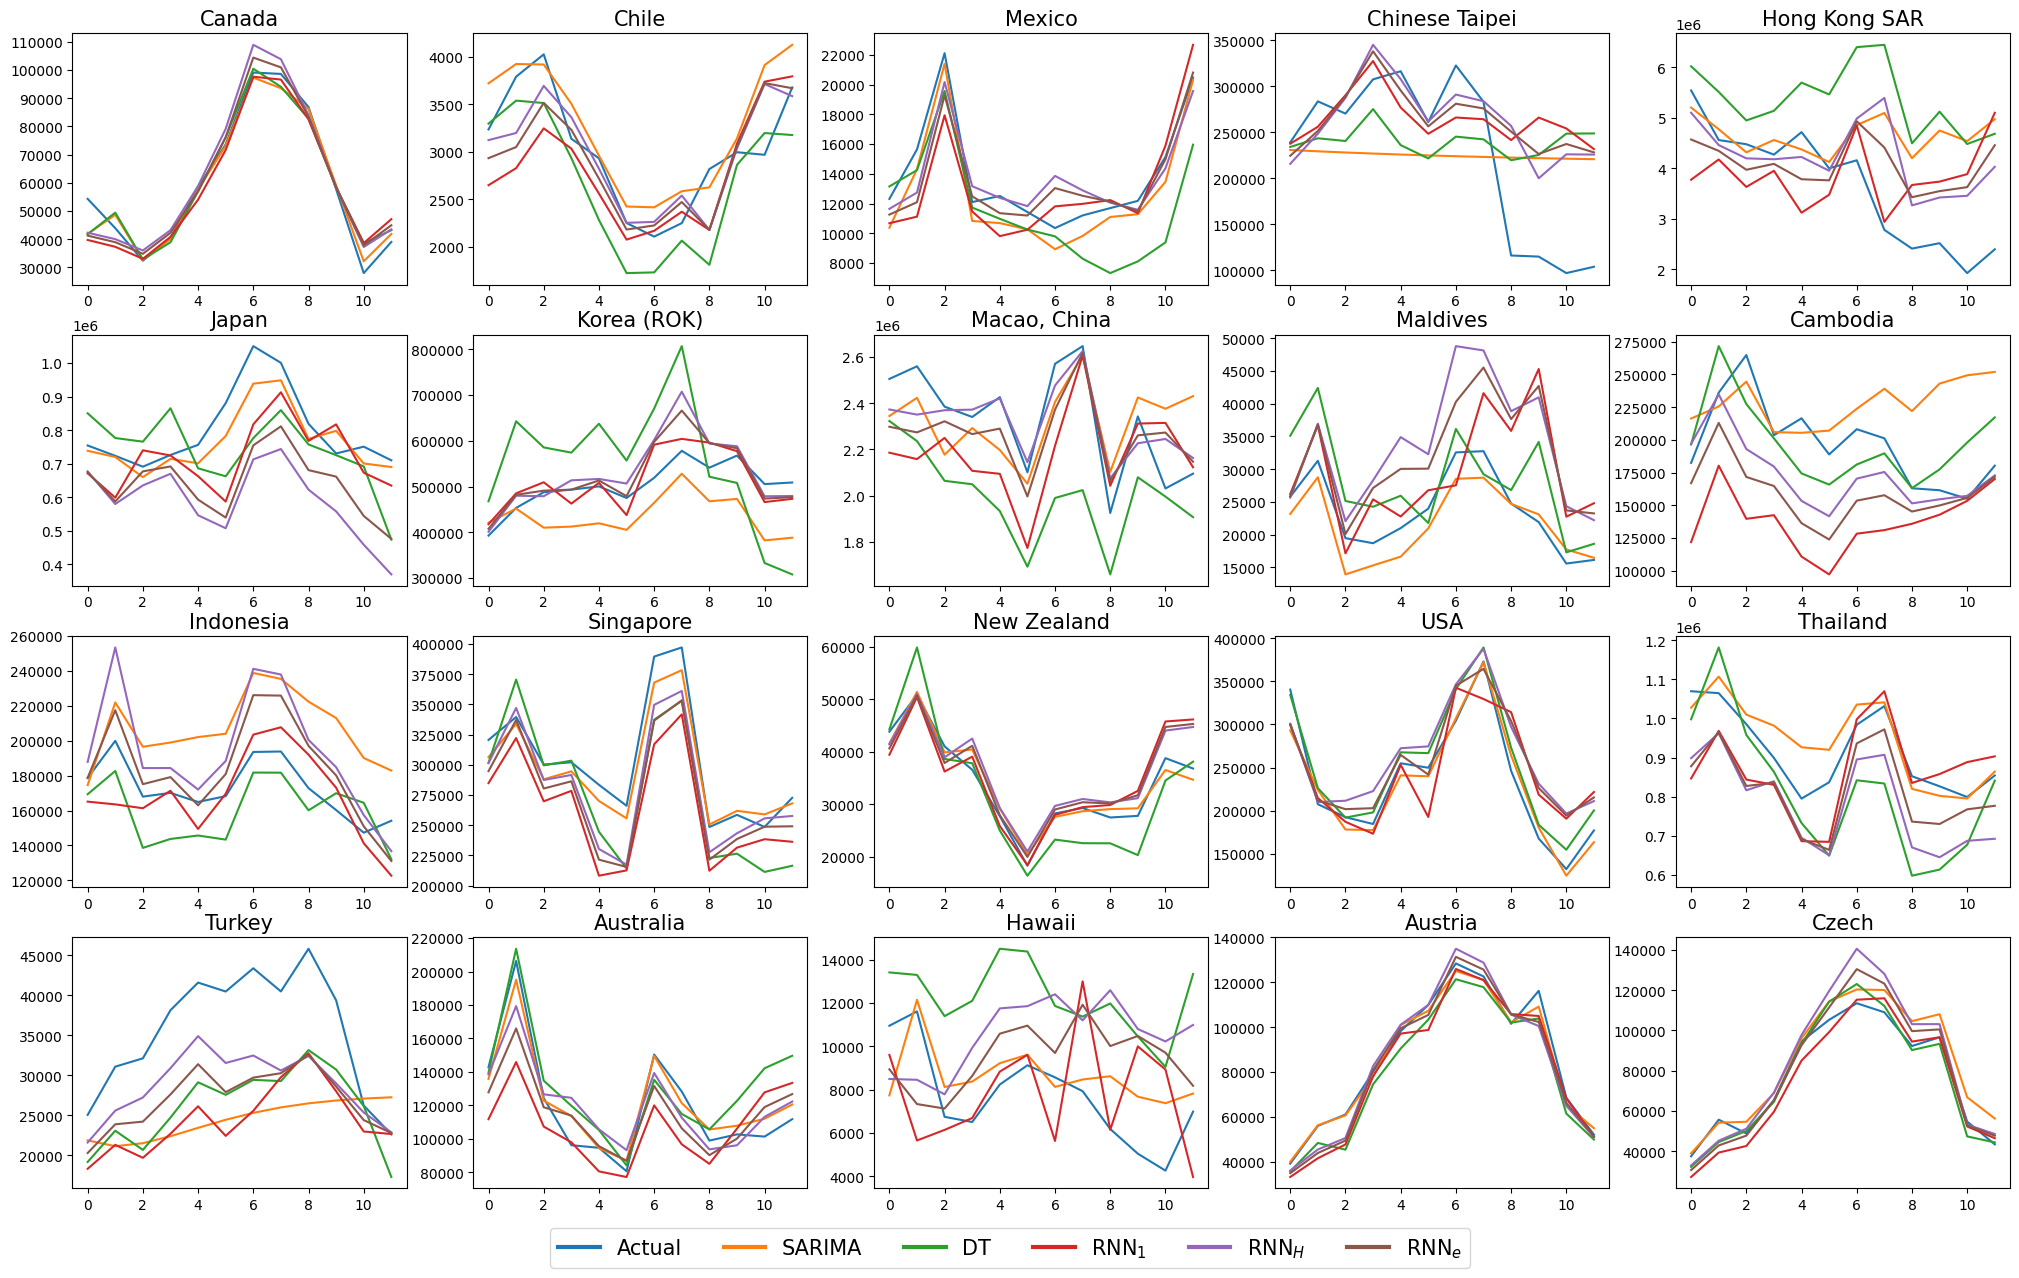
\includegraphics[width=\textwidth]{images/2019 forecasts.png}
         \caption{Forecast prediction of each destination for Experiment 1 (2019).}
     \end{subfigure}
     \vskip\baselineskip
     \begin{subfigure}[b]{\textwidth}
         \centering
         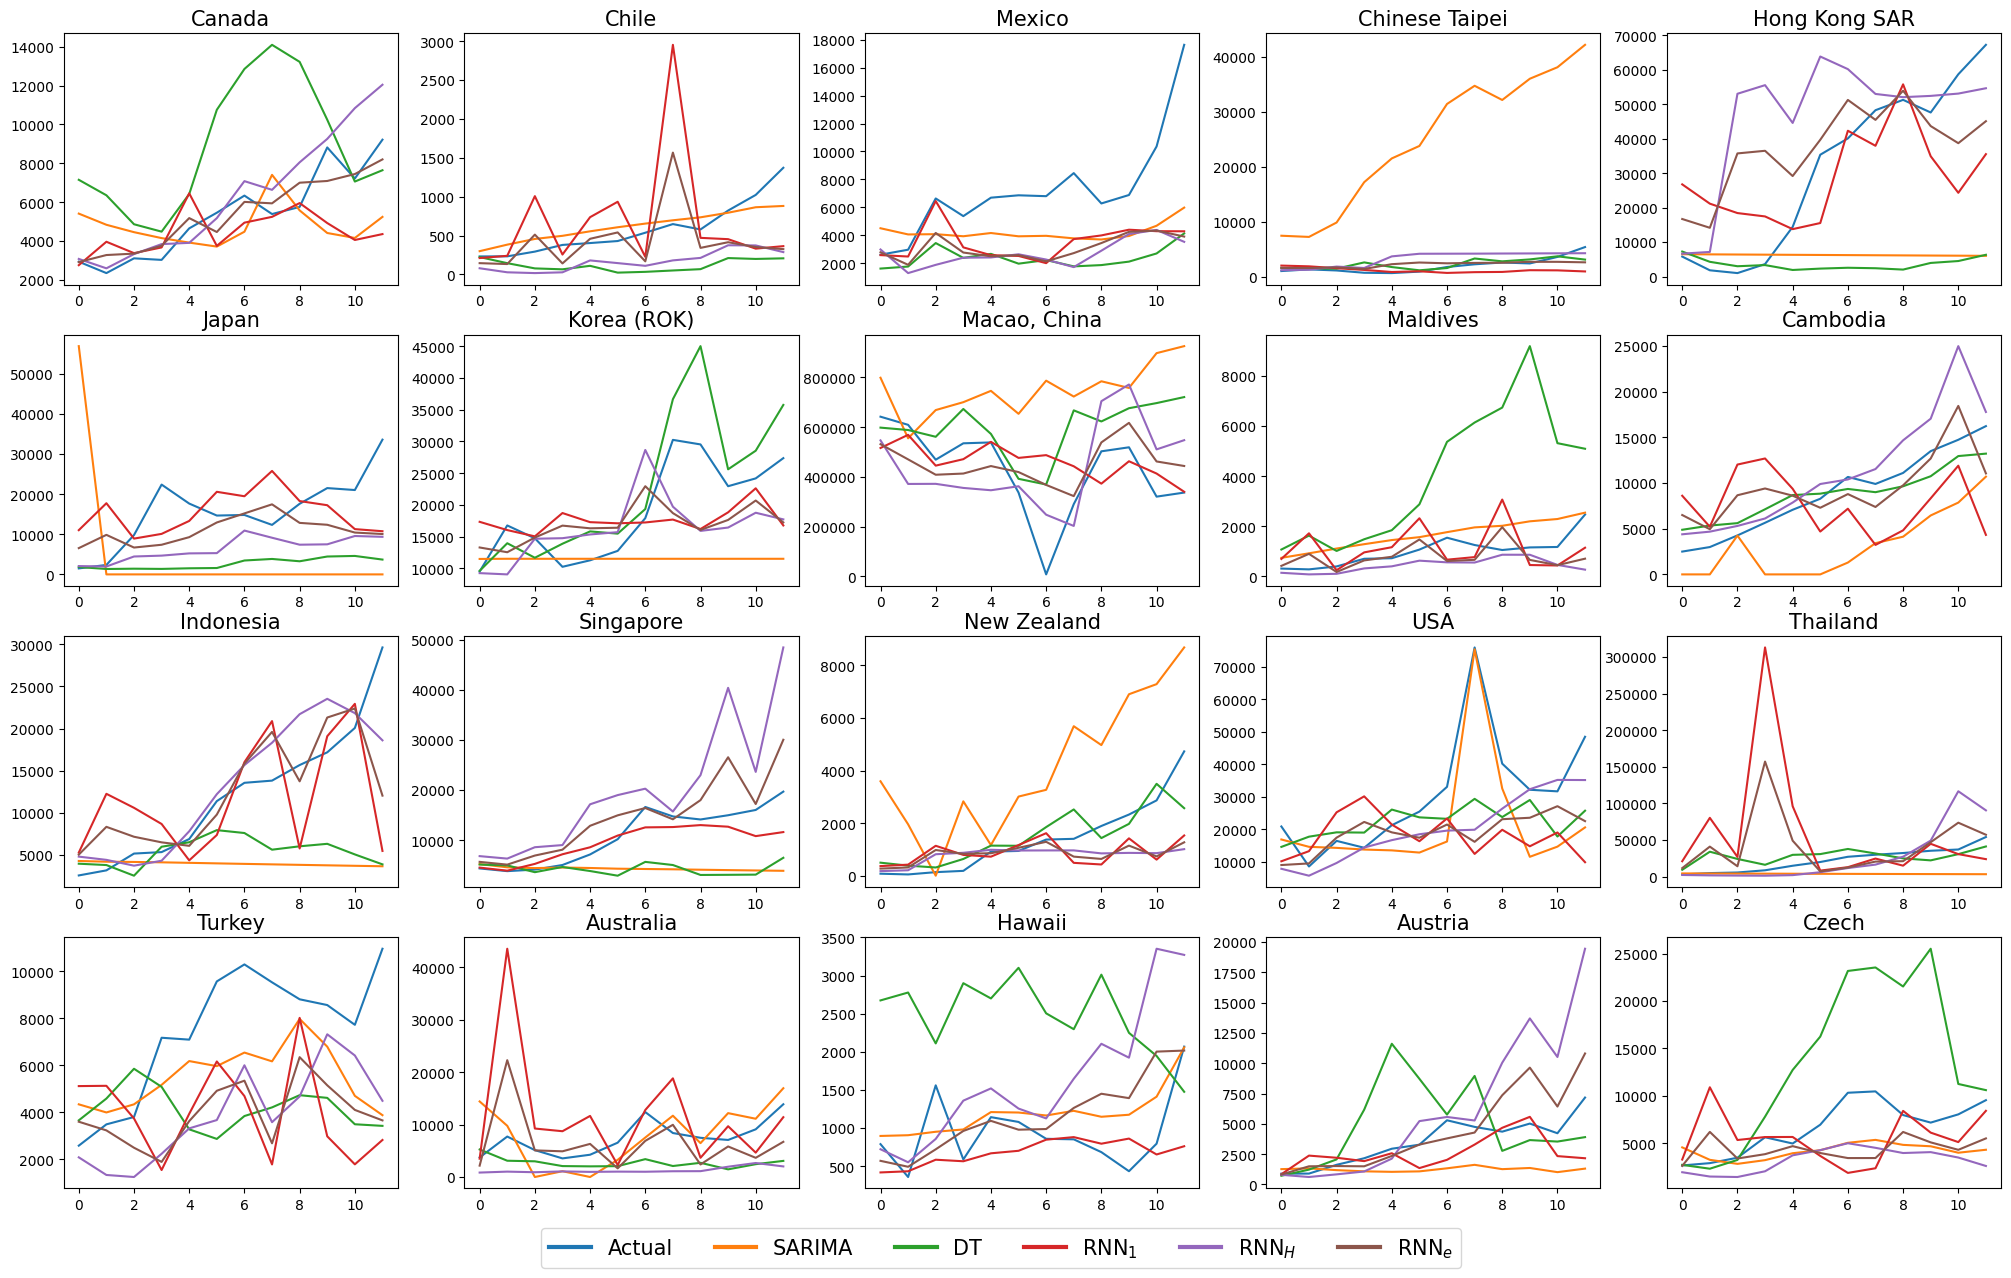
\includegraphics[width=\textwidth]{images/2022 forecasts.png}
         \caption{Forecast prediction of each destination for Experiment 2 (2022).}
     \end{subfigure}
     \caption{X-axis represents the month number in the testing year while the y-axis is the tourist arrival count. Best viewed in colour.}
    \label{fig:expres}
\end{figure}

\section{Discussion}
In Experiment 1, we observed that traditional methods such as SARIMA perform better than other models in terms of MAPE and MASE in Table \ref{table:expres}. This is because there is lesser volatility before the COVID-19 pandemic and the higher number of parameters in RNN causes overfitting as the complexity of the problem is low. Hence, simpler models are preferred when the time series pattern is easier to predict. Conversely, in Experiment 2, RNN models consistently outperform both SARIMA and DT models and should be the preferred model choice when high volatility is expected. Among the RNN models, the ensembling RNN$_e$ model has better overall performance as it has the advantage of both RNN$_1$ and RNN$_H$ models. Figure \ref{fig:expres} visualises the forecast predictions of all models for each destination in both experiments. Finally, to generate the future forecast prediction of tourism arrival from August 2023 to July 2024, we retrain both RNN$_1$ and RNN$_H$ models using all provided training data and the same set of parameters, then ensemble these models to get RNN$_e$ (See \ref{appx:final} for final forecasts).

\section{Conclusion}
To conclude, this work investigates several models and algorithms to forecast tourism arrivals from China to multiple destinations. We proposed an ensembling of an RNN model that produce prediction autoregressively and an RNN model that predicts all required forecasts at once. By experimenting with only pre-COVID-19 data, we found out that traditional methods perform slightly better than deep learning methods due to lesser volatility before the pandemic. However, ensembling RNN models prove to outperform all other methods when evaluating using post-COVID-19 data. 

Several limitations exist in this work. Firstly, assumptions made in this study usually don't hold in the real world. Using a global COVID-19 trend index is unrealistic as different destinations may recover from the pandemic differently. Secondly, without any explanatory variable to model the effect of COVID-19 on Chinese citizens, the model will assume the pandemic is a one-off event without considering the pandemic's impact on people's everyday life. Lastly, China's government policy on travel agencies which are the main contributors of outbound tourists is also not modelled. Future works for further improvement include obtaining more explanatory variables such as natural disasters in each destination, historical flight prices, etc., ensembling using a wider variety of models, using a more sophisticated interval forecasting technique, and employing more recent and advanced architecture such as sequence-to-sequence model, attention mechanism \cite{attention} and possibly transformer models \cite{transformer}.

\newpage

% \bibliographystyle{IEEEtranN}
\printbibliography[segment=0]

\clearpage
\appendix
\newrefsegment %% <== increases the segment number (0 by default)
\section{Appendix}

\subsection{Explanatory Variables}
\label{appx:expvar}
In forecasting problems, the precision of the forecast is usually influenced by other factors. These factors explain the variance of the forecasting variable and are known as explanatory variables. The strength of the correlation between an explanatory variable and the forecasting variable reflects the predictive power of any algorithm used. 
% In the case of tourism forecasting, the explanatory variables include but are not limited to:
% \begin{enumerate}
%     \item Climate of the destination
%     \item Currency exchange rates (FX)
%     \item Economic strength
%     \item Safety and stability of the destination
%     \item Political relationship between source and destination country
% \end{enumerate}
% Certain social or demographic variables such as political relationships are difficult to quantify and require special data processing methods. 
Table \ref{table:expvar} shows the list of explanatory variables and figure \ref{fig:expvar} displays a few examples of the extracted explanatory variables used in this work.

\begin{table}[htbp]
\small
    \centering
        \begin{tabular}{p{0.2\linewidth} |p{0.1\linewidth} |p{0.4\linewidth} |p{0.15\linewidth}}
            Variable & Type & Description & Source \\
            \hline
            \hline
            FX Against China & $\mathbb{R}$ & Monthly currency exchange rate of each destination from Chinese Yuan. & Fxtop.com \cite{FXTop} \\
            \hline
            GDP & $\mathbb{R}^2$ & Yearly total GDP and GDP per capita in constant 2017 USD of each destination and China. & World Bank \cite{worldbank} \\   
            \hline
            FSI & $\mathbb{R}$ & Yearly fragile states index as a safety indicator of each destination. & Fragile States Index \cite{fsi} \\    
            \hline
            Climate & $\mathbb{R}^2$ & Monthly mean temperature and total precipitation of each destination. & CRU \cite{cru} \\    
            \hline
            COVID-19 Situation & $\mathbb{Z}^2$ & Daily COVID-19 cases and deaths for each destination. The daily data is aggregated into monthly frequency by summation. & WHO \cite{covidwho} \\    
            \hline
            COVID-19 Trend & $[0, 100]$ & Worldwide monthly Google Search trend index of the word ``covid" as an indicator of people's interest towards the pandemic. & Google Trends \cite{covidtrend} \\
            \hline
            COVID-19 Travel Policy & $\{0, ..., 4\}$ & International travel control policy of each destination. 0 is no restriction, 1 is screening arrivals, 2 is quarantine arrivals from some regions, 3 is ban arrivals from some regions and 4 means total border closure. & OxCGRT \cite{oxfordcovid} \\
            \hline
            COVID-19 China Internal Movement Policy & $\{0, 1, 2\}$ & Internal movement restriction in China. 0 is no restriction, 1 means recommend to not travel and 2 is movement restriction in place. & OxCGRT \cite{oxfordcovid} \\
            \hline
            Geographic Coordinate & $\mathbb{R}^2$ & Latitude and Longitude of each destination and China. & Google \\
        \end{tabular}
    \caption{Explanatory variables and their data source.}
    \label{table:expvar}
\end{table}

Furthermore, feature engineering is also performed to create several features based on domain knowledge. Table \ref{table:feateng} shows the new features derived from the extracted explanatory variables. Since the engineered features are highly correlated to the extracted explanatory variables, we removed the raw explanatory variables such as total GDP, total GDP per capita and geographic coordinate to reduce collinearity. As described in Section \ref{sect:shocks}, special care has been taken to model them: (1) ``Travel Restriction'' is set to 1 for Korea (ROK) between March and November 2017 as China bans travel agencies from selling package tours to Korea (ROK), and set to 1 for Chinese Taipei starting from September 2019 to January 2024 as China bans individual travel permits to Chinese Taipei and we assumed that their political relationship will improve after Chinese Taipei's 2024 presidential election; (2) ``Unrest'' is set to 1 for all destinations between April to July 2003 due to SARS outbreak, set to 1 for Singapore and Thailand between April 2014 and January 2015 because of aviation incidents of Malaysian Airlines aircraft, set to 1 for Turkey from December 2015 to February 2017 due to 2016 Turkish coup d'état attempt, and set to 1 for Hong Kong (SAR) from August 2019 to June 2020 because of protests and demonstrations.

\begin{table}[htbp]
\small
    \centering
        \begin{tabular}{p{0.25\linewidth} |p{0.05\linewidth} |p{0.6\linewidth}}
            Variable & Type & Description \\
            \hline
            \hline
            GDP and GDP per capita Ratio & $\mathbb{R}^2$ & GDP and GDP per capita of each destination divided by GDP and GDP per capita of China respectively. \\
            \hline
            GDP and GDP per capita Growth Difference & $\mathbb{R}^2$ & Percentage growth of destination minus percentage growth of China for both GDP and GDP per capita. \\
            \hline
            Month $\sin$ and $\cos$ & $\mathbb{R}^2$ & See Figure \ref{fig:monthfeat}. \\
            \hline
            Popularity & $\mathbb{R}$ & Median visitor arrivals of each destination as popular destinations may exhibit different trends compared to unpopular ones. \\
            \hline
            Travel Restriction & $\{0, 1\}$ & Boolean feature to indicate the freedom of Chinese citizens to travel to each destination. By default it is set to 0 if ``COVID-19 China Internal Movement Policy'' and destination's ``COVID-19 Travel Policy'' is 0, otherwise it is set to 1. \\
            \hline
            Unrest & $\{0, 1\}$ & Boolean feature to indicate feelings of unrest due to shocks or unusual events. \\
            \hline
            Distance from China & $\mathbb{R}$ & Geodesic distance in kilometres calculated using latitude and longitude of each destination and China. \\
            \hline
        \end{tabular}
    \caption{Engineered features and their description.}
    \label{table:feateng}
\end{table}

\begin{figure}
     \centering
     \begin{subfigure}[b]{0.42\textwidth}
         \centering
         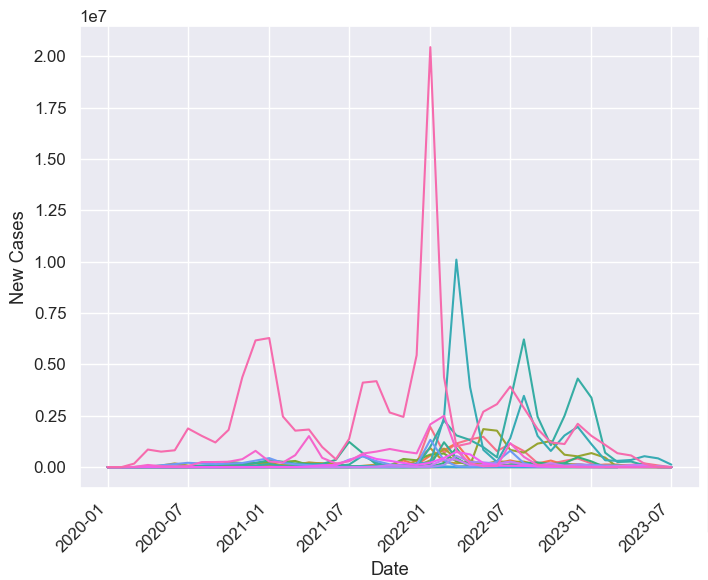
\includegraphics[width=\textwidth]{images/monthly covid.png}
         \caption{Monthly new COVID-19 cases}
     \end{subfigure}
     \begin{subfigure}[b]{0.55\textwidth}
         \centering
         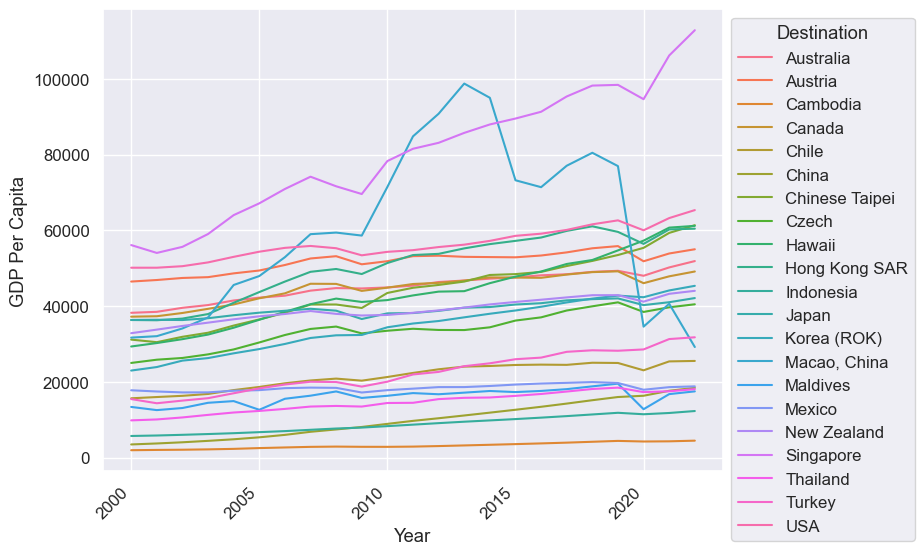
\includegraphics[width=\textwidth]{images/yearly gdp per capita.png}
         \caption{Yearly GDP per capita}
     \end{subfigure}
     \vskip\baselineskip
     \begin{subfigure}[b]{0.42\textwidth}
         \centering
         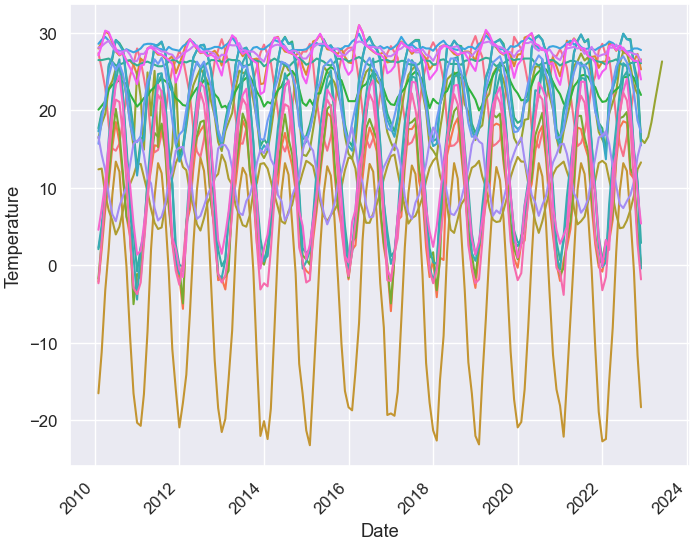
\includegraphics[width=\textwidth]{images/monthly temperature.png}
         \caption{Monthly mean temperature (\degree C)}
     \end{subfigure}
     \begin{subfigure}[b]{0.55\textwidth}
         \centering
         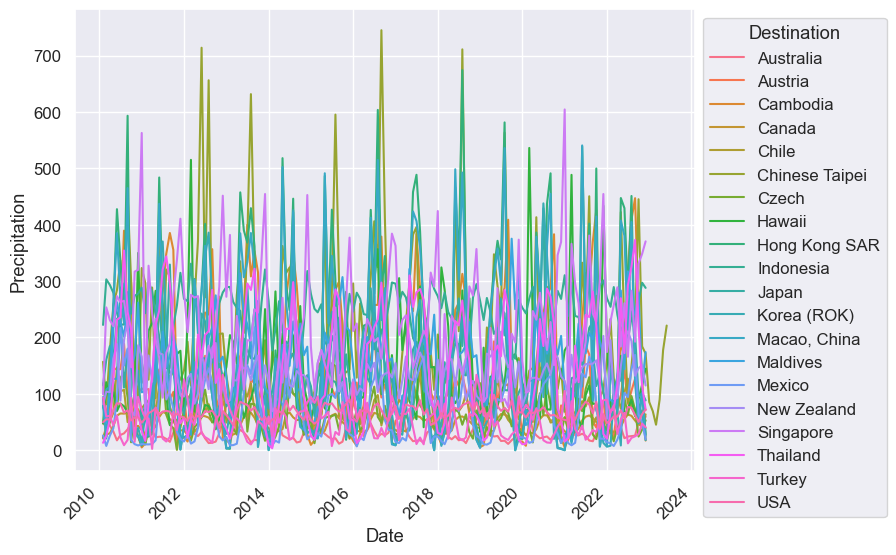
\includegraphics[width=\textwidth]{images/monthly precipitation.png}
         \caption{Monthly total precipitation (mm)}
     \end{subfigure}
    \caption{Example plots of explanatory variables for each destination. Best viewed in colour.}
    \label{fig:expvar}
\end{figure}

Lastly, explanatory variables are forecasted to obtain future values with simple methods. GDP and GDP per capita are forecasted with exponential smoothing \cite{winterexp1960} while ``FX against China'' and FSI are predicted using other variables with an ensemble of ARIMA and decision tree. COVID-19 variables (i.e. ``COVID-19 Situation'' and ``COVID-19 Trend'') are projected by halving them every timestep until they reach zero. Other variables like ``COVID-19 Travel Policy'', ``Travel Restriction'', ``Unrest'', etc are set to zero.

\subsection{Conditioning Prediction with Hidden State Initialisation}
\label{appx:cond}
There are several ways to initialise the hidden state based on different conditions. For example, one may set a random initial hidden state for each condition and allow model training to update these initial hidden states with backpropagation. In our work, we chose to initialise hidden states based on FastText \cite{fasttext}, a pretrained word representation model that is able to output an embedding vector given a word. First, we perform dimensionality reduction on the embeddings using PCA to reduce the dimension from 300 to the desired hidden state dimension. Then, we retrieve the word vector embedding of each destination's name and use them as the initial hidden states. These hidden states are frozen and not updated during model training. The idea is that the pretrained FastText model had learnt the similarity between each destination and represented them in the embeddings. Figure \ref{fig:fasttext} shows the FastText embeddings of each destination where we used t-SNE \cite{tsne} to further reduce the dimension to 2 for easier visualisation. It can be observed that similar destinations (e.g. USA, Hawaii and Canada) are usually closer to each other or have small cosine distances in the 2D space.

\begin{figure}[htbp]
     \centering
     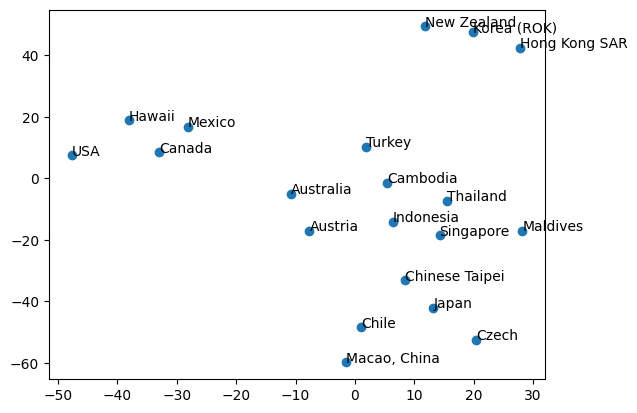
\includegraphics[width=.5\textwidth]{images/fasttext embeddings.png}
     \caption{Visualisation of FastText embeddings reduced to 2 dimensions using t-SNE.}
    \label{fig:fasttext}
\end{figure}

\subsection{Evaluation Metrics}
\label{appx:metric}
Evaluation metrics used for point forecasts of one destination are RMSE, R2, MAE, MAPE and MASE with mathematical formulation given as follows:
\[
\begin{split}
    {RMSE} &= \sqrt{\frac{\sum_{t=N+1}^{N+H} (y_t - \hat{y}_t)^2}{H}} \\
    {R2} &= 1 - \frac{\sum_{t=N+1}^{N+H} (y_t - \hat{y}_t)^2}{(y_t - \Bar{y}) ^ 2} \\
    {MAE} &= \frac{\sum_{t=N+1}^{N+H} |y_t - \hat{y}_t|}{H} \\
    {MAPE} &= \frac{1}{H} \sum_{t=N+1}^{N+H} \frac{|y_t - \hat{y}_t|}{y_t} \\
    {MASE} &= \frac{1}{H} \sum_{t=N+1}^{N+H} \frac{|y_t - \hat{y}_t|}{\frac{1}{t-H-m} \sum_{i=m+1}^{t-H} |y_i - y_{i-m}|} \\
\end{split}
\]
where $N$ is the number of historical data, $H$ is the forecast horizon, $y_t$ is the actual ground truth at time $t$, $\hat{y}_t$ is the point forecast prediction at time $t$, $\Bar{y}$ is the mean of all actual ground truth in the forecast period and $m$ is the seasonal period. To evaluate interval forecast, we use Winkler score \cite{winkler} with the following definition:
\[{Winkler} = 
\begin{cases}
    w_t & l_t \leq y_t \leq u_t \\
    w_t + 2(l_t-y_t)/\alpha & l_t > y_t \\
    w_t + 2(y_t - u_t)/\alpha & u_t < y_t \\
\end{cases}
\]
where $l_t$ and $u_t$ are the lower and upper value of the forecast interval respectively, $w_t$ is $u_t - l_t$ and $\alpha$ is $1-c$ (i.e. $\alpha=0.2$). The mean Winkler score is simply the average Winkler score for all predicted intervals in the forecast period.

\subsection{Hyperparameter Tuning with Grid Search}
\label{appx:params}
For SARIMA, the tunable parameters are $p$, $d$, $q$, $P$, $D$ and $Q$ while the seasonal period $m$ is set to 12. For DT, the tunable parameters include model type (i.e. RF or XGBoost), number of trees to build and max tree depth while for RNN, they include model type (i.e. LSTM or GRU), length of the input sequence, number of RNN layers, hidden size, learning rate, etc. Since the number of hyperparameters and training time are relatively small, we employed grid search with cross-validation for hyperparameter tuning. Each possible pair of parameters are trained on all cross-validation splits and the parameters with the lowest average RMSE across all validation splits are selected. Table \ref{table:params} outlines the search space of the hyperparameters and the final selected parameters for DT and RNN models. The best input sequence length found with grid search is 24 timesteps while the model performance gets progressively worse the longer the input sequence is. This is due to the ``forgetting" phenomenon in RNN. As the input sequence gets longer, the RNN model gradually forgets the conditioning hidden state at the first timestep. Figure \ref{fig:inputlen} highlights the effects of the length of the input sequence on the final model performance. The number of training instances decreases as a longer input sequence is used which may also be one of the reasons RMSE become progressively worse. ``Full" in Table \ref{table:params} and Figure \ref{fig:inputlen} refers to training with the longest possible input sequence. 

\begin{table}[htbp]
    \centering
        \begin{tabular}{l|l|l|l}
            Model & Parameter & Search Space & Best Value \\
            \hline
            \multirow{3}{*}{DT} & Model Type & \{RF, XGBoost\} & XGBoost \\
                    & Number of Trees & \{10, 50, 100, 150, 200, 250, 300, 500\} & 250 \\
                    & Max tree depth & [3, 10] & 6 \\
            \hline
            \multirow{6}{*}{RNN} & Model Type & \{LSTM, GRU\} & GRU \\
                    & Length of input sequence & \{12, 24, 36, 48, 60, Full\} & 24 \\
                    & Number of layers & [1, 5] & 3 \\
                    & Hidden size & \{20, 40, 50, 60, 75, 100\} & 50 \\
                    & Optimizer type & \{RMSprop, NAdam\} & RMSprop \\
                    & Learning rate & \{0.01, 0.005 0.001, 0.0005, 0.0001\} & 0.0005 \\
        \end{tabular}
    \caption{Hyperparameter search space and best value for DT and RNN models.}
    \label{table:params}
\end{table}

\begin{figure}[htbp]
     \centering
     \begin{subfigure}[b]{.43\textwidth}
         \centering
         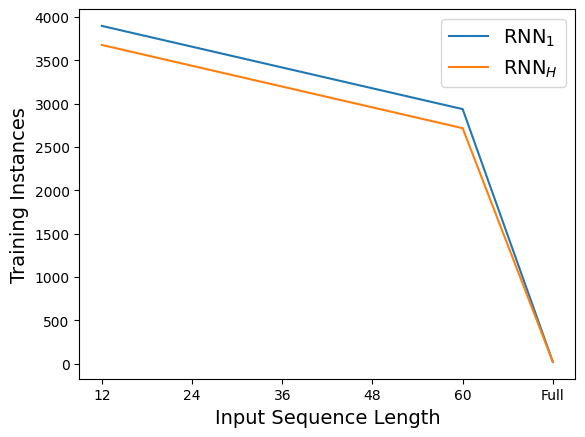
\includegraphics[width=\textwidth]{images/input length training instances.png}
         \caption{Effects of input sequence length on number of training instances.}
     \end{subfigure}
     \hfill
     \begin{subfigure}[b]{.45\textwidth}
         \centering
         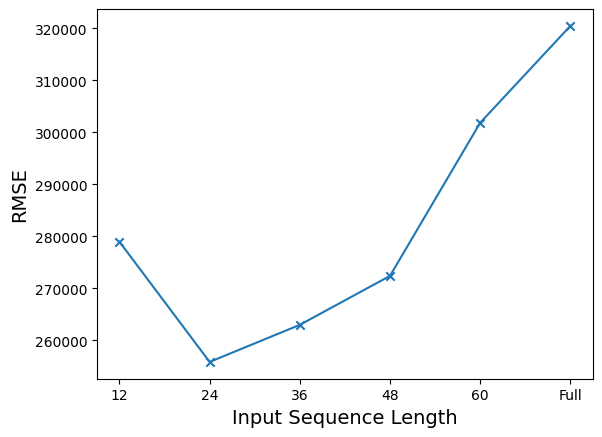
\includegraphics[width=\textwidth]{images/input length.png}
         \caption{Effect of input sequence length on the RMSE of RNN$_e$ model.}
     \end{subfigure}
     \caption{X-axis represents the length of the input sequence used in Experiment 1 (2019).}
     \label{fig:inputlen}
\end{figure}

\subsection{Ablation Studies on Encoding Temporal Features}
\label{appx:ablation}
In this section, we performed ablation studies on the choice of encoding method for periodical temporal features. Common ways to encode them include one-hot encoding, ordinal encoding and using cyclical features to encode temporal features (See \ref{fig:monthfeat}). Table \ref{table:ablation} shows the evaluation metrics of model RNN$_e$ in Experiment 1 (2019) point forecast using different types of encoding methods. Although temporal features like month numbers are highly correlated with climate features, it is not always true for destinations near the equator such as Singapore or Indonesia. As seen in Table \ref{table:ablation}, an attempt to reduce collinearity by not using any temporal features gives the worst performance in terms of RMSE and R2. Ordinal encoding is not suitable as there is no continuity between the beginning and end of periodic temporal features while one-hot encoding will result in more features and thus increase the risk of overfitting. Finally, encoding with cyclical features gives the best performance and is used in our final model.
% However, 

\begin{table}[htbp]
\small
    \centering
        \begin{tabular}{l|ccccc}
            Encoding Method & RMSE ($\downarrow$) & R2 ($\uparrow$) & MAE ($\downarrow$) & MAPE ($\downarrow$) & MASE ($\downarrow$) \\
            \hline
            No Temporal Feature & 292387 & 0.901 & 84835 & 0.185 & 1.976 \\
            Ordinal Encoding & 288702 & 0.904 & 94801 & 0.205 & 2.172 \\
            One-Hot Encoding & 263614 & 0.920 & 87592 & 0.176 & 2.036 \\
            Cyclical Encoding & \textbf{255846} & \textbf{0.924} & \textbf{79243} & \textbf{0.169} & \textbf{1.781} \\
        \end{tabular}
    \caption{Ablation studies on the choice of encoding method for periodical temporal features for RNN$_e$ model in Experiment 1 (2019). Lower is better for all metrics except R2.}
    \label{table:ablation}
\end{table}

\subsection{Final Forecasts}
\label{appx:final}
For each destination, we are required to forecast up to July 2024. To achieve that, we retrained the RNN models using all training data provided without changing the best parameters found using grid search in \ref{appx:params}. Point forecast predictions are the ensemble of both RNN models (i.e. RNN$_e$) while interval forecast predictions are approximated with 100 Monte-Carlo sampling. Figure \ref{fig:final} presents the final point forecast and interval forecast of tourist arrivals for each destination.

\begin{figure}
     \centering
     \begin{subfigure}[b]{\textwidth}
         \centering
         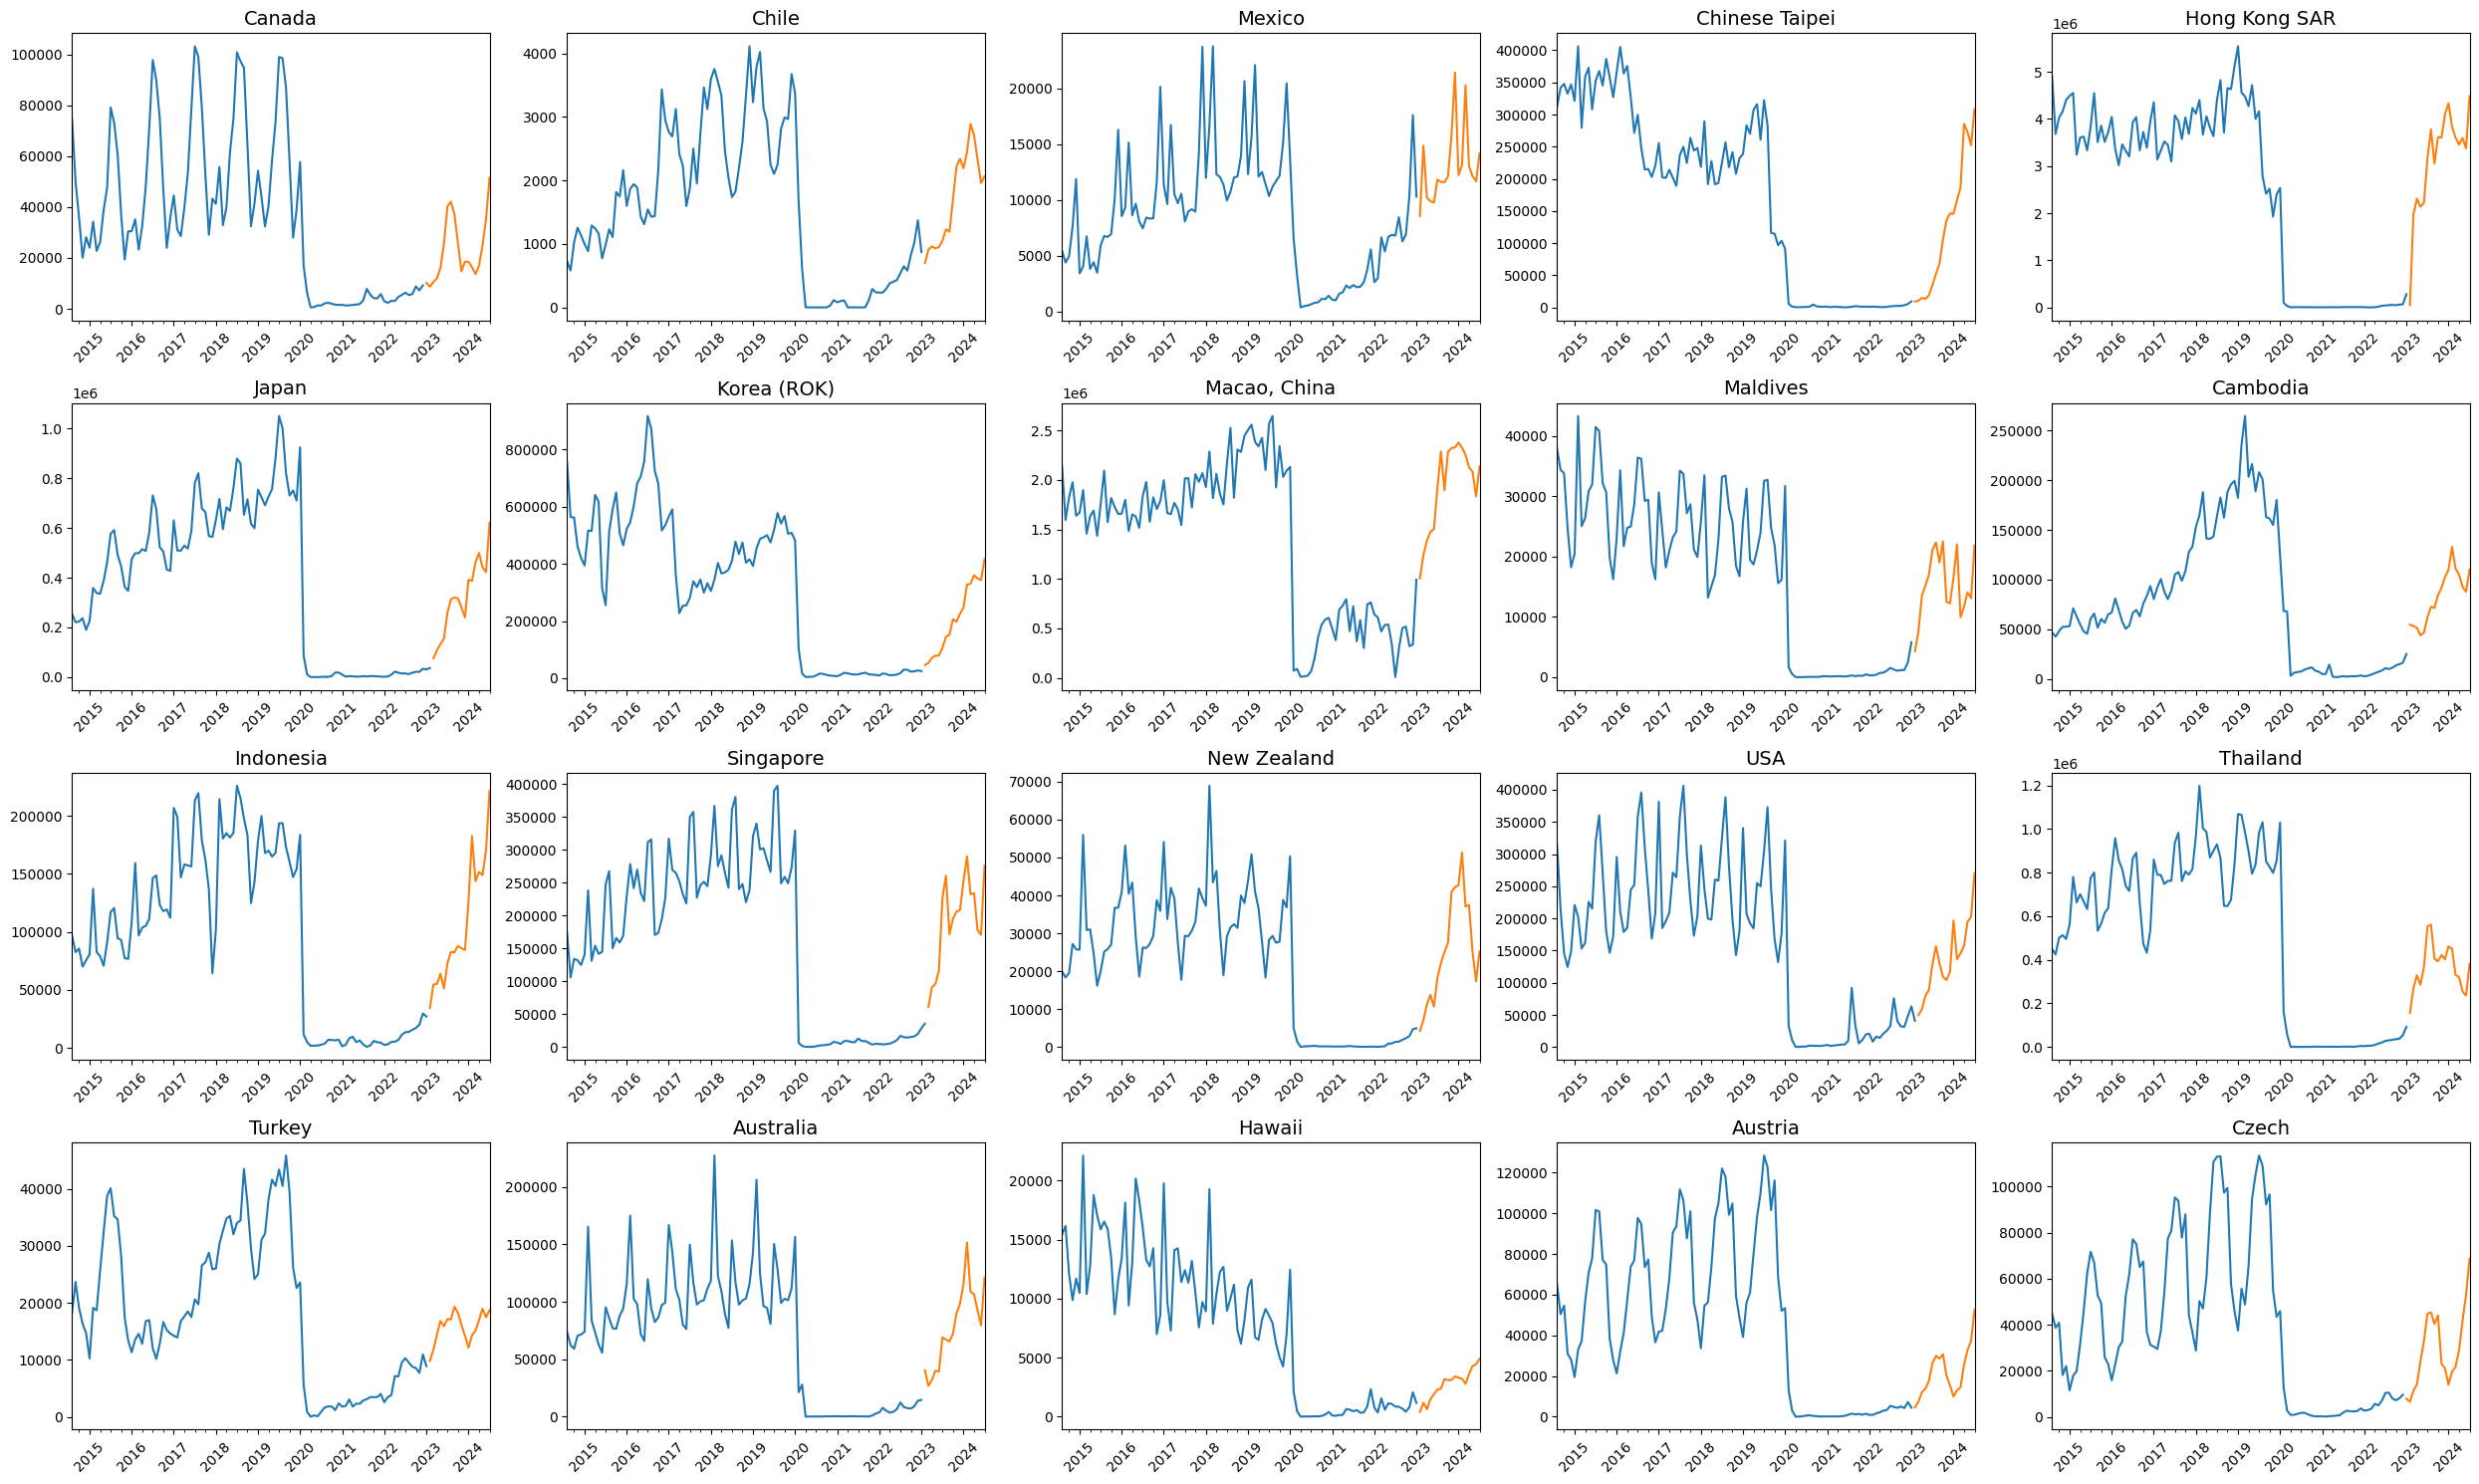
\includegraphics[width=\textwidth]{images/final point.png}
         \caption{Point forecast prediction for each destination where the blue line indicates the actual data and the orange line indicates the forecasts.}
     \end{subfigure}
     \vskip\baselineskip
     \begin{subfigure}[b]{\textwidth}
         \centering
         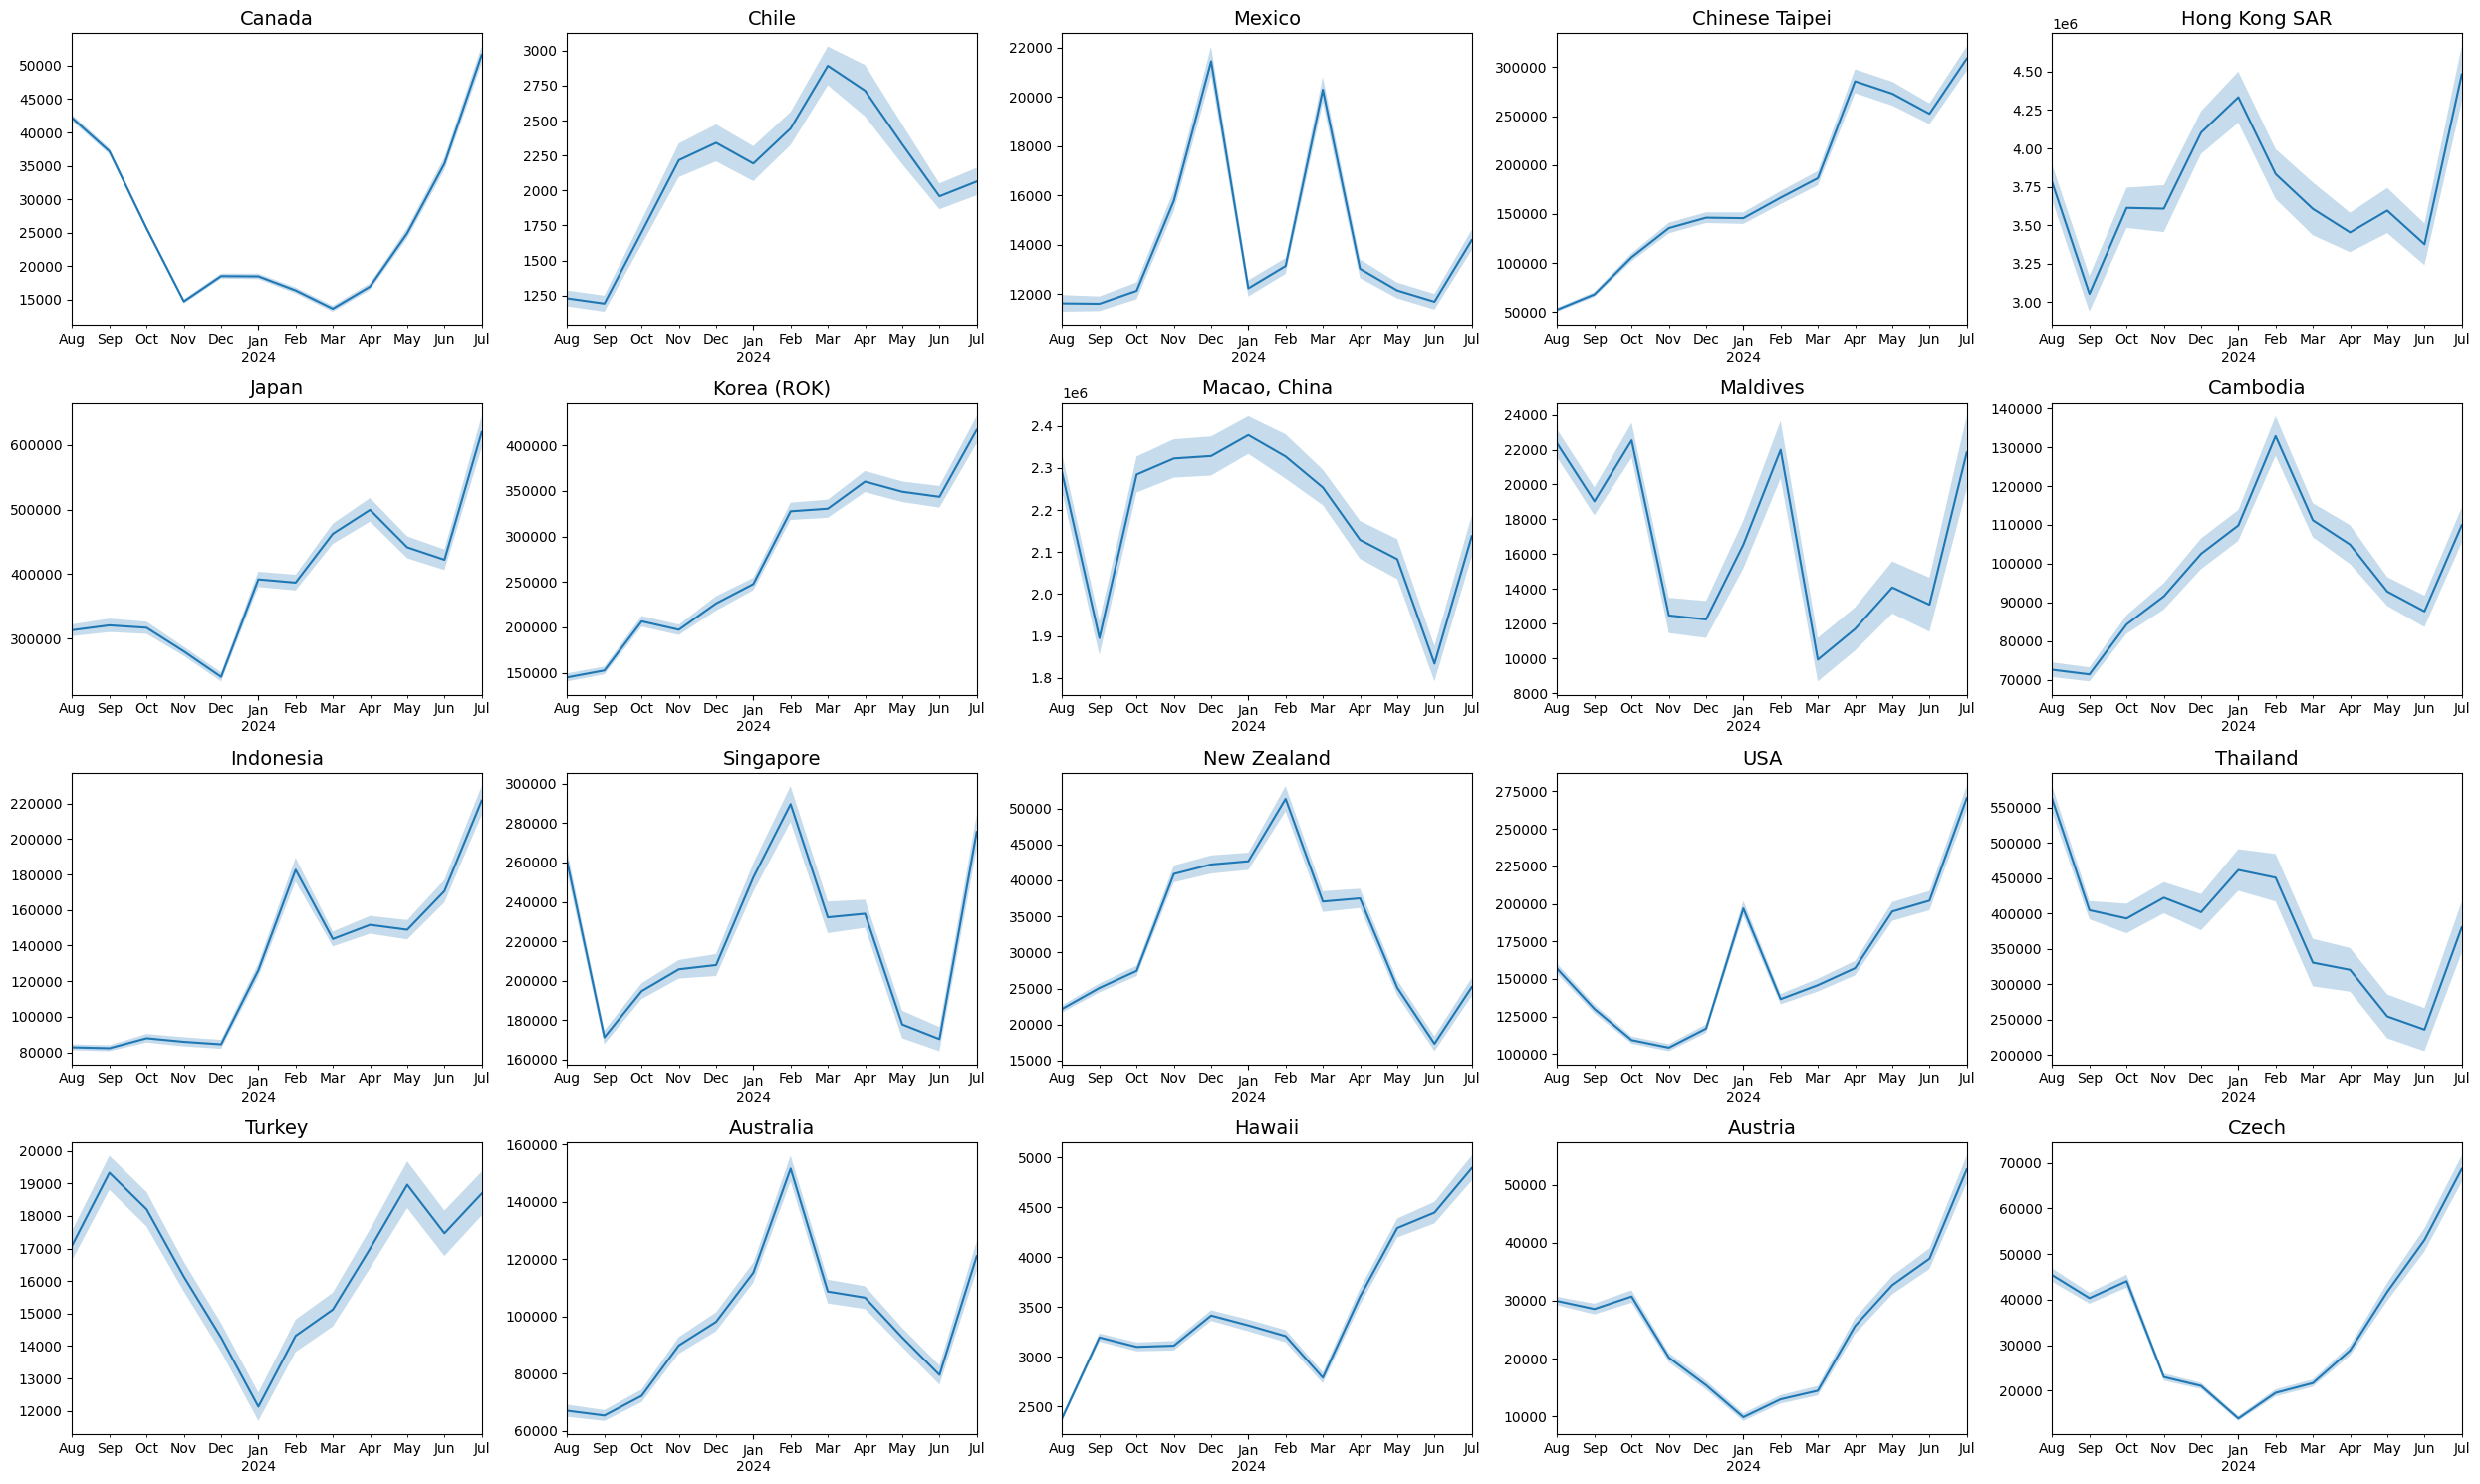
\includegraphics[width=\textwidth]{images/final interval.png}
         \caption{Interval forecast prediction for each destination where the shaded region shows the 80\% confidence interval.}
     \end{subfigure}
     \caption{X-axis represents the date (month and year) while the y-axis is the tourism arrival count.}
    \label{fig:final}
\end{figure}

\clearpage
\printbibliography[heading=subbibliography,filter=appendixOnlyFilter]

\end{document}